\documentclass[9pt,pdf,hyperref={unicode}]{beamer}
\beamertemplatenavigationsymbolsempty

\setbeamertemplate{blocks}[rounded=true, shadow=true]
\setbeamertemplate{footline}[page number]
\usepackage{multicol}

\usefonttheme{serif}

\usepackage[utf8]{inputenc}
\usepackage[english, russian]{babel}
\usepackage{amsmath,mathrsfs,mathtext}
\usepackage{graphicx, epsfig}
\usepackage{caption}
\usepackage{subfig}
\usepackage{amsmath, bm}

\usepackage{comment}

\usepackage{tabularx}

\usepackage{tikz}

\DeclareMathOperator*{\argmin}{arg\,min}
\DeclareMathOperator*{\argmax}{arg\,max}

\makeatletter
\let\@@magyar@captionfix\relax
\makeatother

\usetheme{Warsaw}
\usecolortheme{sidebartab}
\definecolor{beamer@blendedblue}{RGB}{31,96,49}

\setbeamertemplate{enumerate items}[circle]

\setbeamersize{text margin left=1.5em, text margin right=1.5em}

\usepackage{ragged2e}


%----------------------------------------------------------------------------------------------------------
\title[\hbox to 56mm{Смесь экспертов \hfill\insertframenumber\,/\,\inserttotalframenumber}]
{Смеси экспертов}
\author[А.\,В.~Грабовой]{\large \\Грабовой Андрей Валериевич}
\institute{\large
Московский физико-технический институт}

\date{\footnotesize{МФТИ, г. Долгопрудный}}
%----------------------------------------------------------------------------------------------------------
\begin{document}
%----------------------------------------------------------------------------------------------------------
\begin{frame}
\titlepage
\end{frame}

%----------------------------------------------------------------------------------------------------------
\begin{frame}{План}
	\begin{enumerate}
		\item ЕМ--алгоритм:
			\begin{itemize}
				\item Классический,
				\item Вариационный,
			\end{itemize}
		\item Смесь моделей:
			\begin{itemize}
				\item Постановка задачи,
				\item Итерационные формулы полученные при помощи вариационного ЕМ--алгоритма,
				\item Илюстрация сходимости,
			\end{itemize}
		\item Смесь экспертов
			\begin{itemize}
				\item Постановка задачи,
				\item Итерационные формулы полученные при помощи вариационного ЕМ--алгоритма,
				\item Илюстрация сходимости,
			\end{itemize}
	\end{enumerate}
\end{frame}

%----------------------------------------------------------------------------------------------------------
\begin{frame}{Вариационный ЕМ--алгоритм}
\justifying
	Максимизация обоснованости:
	\begin{equation}
	\label{sl:1:eq:1}
		\begin{aligned}
			\bm{\Theta} = \arg\max_{\bm{\Theta}} p\left(\textbf{y}|\textbf{X}, \bm{\Theta}\right)
		\end{aligned}
	\end{equation}
	ELBO:
	\begin{equation}
	\label{sl:1:eq:2}
		\begin{aligned}
			\mathcal{L}\left(q\bigr(\textbf{Z}\bigr), \bm{\Theta}\right)&= \int q\bigr(\textbf{Z}\bigr)\log\frac{p\left(\textbf{y}, \textbf{Z}|\bm{\Theta}, \textbf{X}\right)}{q\left(\textbf{Z}\right)}d\textbf{Z}\\
			&=p\left(\textbf{y}|\textbf{X}, \bm{\Theta}\right) - \mathsf{D}_{KL}\left(q\bigr(\textbf{Z}\bigr)||p\bigr(\textbf{Z}|\textbf{y}, \textbf{X}, \bm{\Theta}\bigr)\right)
		\end{aligned}
	\end{equation}
	ЕМ--алгоритм:
	\begin{enumerate}
		\item Е--шаг: 
			\begin{equation}
			\label{sl:1:eq:3}
				\begin{aligned}
					q^{s}\bigr(\textbf{Z}\bigr) = \arg\max_{q\bigr(\textbf{Z}\bigr)\in Q} \mathcal{L}\left(q\bigr(\textbf{Z}\bigr), \bm{\Theta}^{s-1}\right)		
				\end{aligned}
			\end{equation}
		\item М--шаг: 
			\begin{equation}
			\label{sl:1:eq:4}
				\begin{aligned}
					\bm{\Theta}^{s} = \arg\max_{\bm{\Theta}} \mathcal{L}\left(q^{s}\bigr(\textbf{Z}\bigr), \bm{\Theta}\right)		
				\end{aligned}
			\end{equation}
	\end{enumerate}
	
	Вариационный ЕМ--алгоритм (Mean Field Approximation\footnote[1]{\url{https://github.com/andriygav/EMprior/blob/master/Lecture/Grabovoy2019MeanField.pdf}}):
	\begin{enumerate}
		\item Е--шаг: 
			\begin{equation}
			\label{sl:1:eq:5}
				\begin{aligned}
					\log q\left(\textbf{Z}_{k}^{s}\right) \propto \mathsf{E}_{q/k}\log p\left(\textbf{y}, \textbf{Z}|\textbf{X},\bm{\Theta}^{s-1}\right)
				\end{aligned}
			\end{equation}
		\item М--шаг: 
			\begin{equation}
			\label{sl:1:eq:6}
				\begin{aligned}
					\bm{\Theta}^{s} = \arg\max_{\bm{\Theta}} \mathbf{E}_{q^{s}}\log p\left(\textbf{y}, \textbf{Z}|\textbf{X},\bm{\Theta}\right)
				\end{aligned}
			\end{equation}
	\end{enumerate}

\end{frame}
%----------------------------------------------------------------------------------------------------------
\begin{frame}{Смесь моделей}
\justifying
\begin{definition}
Смесь моделей~---~мультимодель, ответы которой представляют собой взвешенную сумму ответов всех задействованных моделей независимо от объекта.

\begin{equation}
\label{sl:2:eq:1}
	\begin{aligned}
		\hat{\textbf{f}} = \sum_{k=1}^{K}\pi_{k}\textbf{f}_k, \qquad \pi_{k} = const, \quad \sum_{k=1}^{K}\pi_{k} = 1,
	\end{aligned}
\end{equation}
где~$\textbf{f}$~---~мультимодель, а $\textbf{f}_k$~---~локальная модель.
\end{definition}

{\bf Пример 1}:
\begin{enumerate}
	\item Веса моделей в смеси~$\bm{\pi}$ получены из априорного распределения 
		\begin{equation}
		\label{sl:2:eq:2}
			\begin{aligned}
				p\left(\bm{\pi}|\mu\right);
			\end{aligned}
		\end{equation}
	\item Вектора параметров~$\textbf{w}_k$ получены из нормального распределения 
		\begin{equation}
		\label{sl:2:eq:3}
			\begin{aligned}
				p\left(\textbf{w}_k|\textbf{A}_k\right) = \mathcal{N}\left(\textbf{w}_k|\textbf{0}, \textbf{A}_{k}\right),~k=1,\cdots K;
			\end{aligned}
		\end{equation}
		
	\item Для каждого объекта~$\textbf{x}_i$ существует модель~$\textbf{f}_{k_i},$ которой он описывается, причем $p\left(k_i=k\right) = \pi_k;$
	
	\item  Для каждого объекта $\textbf{x}_i$ класс $y_i$ определен в соответсвии с моделью 
		\begin{equation}
		\label{sl:2:eq:3}
			\begin{aligned}
				\textbf{f}_{k_i}:~y_i\sim~\mathcal{N}\left(\textbf{w}_{k_i}^{\mathsf{T}}\textbf{x}_i + b_k, \beta^{-1}\right)
			\end{aligned}
		\end{equation}
\end{enumerate}

\end{frame}
%----------------------------------------------------------------------------------------------------------
\begin{frame}{Пример 1}
\justifying
Правдоподобие модели:
	\begin{equation}
	\label{sl:3:eq:1}
		\begin{aligned}
			p(\textbf{y}, \textbf{W}, \bm{\pi}|\textbf{X}, \textbf{A}, \beta, \bm{\mu}) = \text{Dir}(\bm{\pi}|\bm{\mu})
			\prod_{k=1}^{K}N(\textbf{w}_k|\textbf{0}, \textbf{A}_k)
			\prod_{i=1}^{N}\left(\sum_{k=1}^{K}\pi_k\mathcal{N}(y_i|\textbf{w}_k^{\mathsf{T}}\textbf{x}_i, \beta^{-1})\right)
		\end{aligned}
	\end{equation}
Введем скрытые переменные $\textbf{Z} = ||z_{ik}||,$ где $~z_{ik} = 1 \Leftrightarrow k_i=k$:
	\begin{equation}
	\label{sl:3:eq:2}
		\begin{aligned}
			p(\textbf{y}, \textbf{W}, \bm{\pi}, \textbf{Z}|\textbf{X}, \textbf{A}, \beta, \bm{\mu}) = \text{Dir}(\bm{\pi}|\bm{\mu})
			\prod_{k=1}^{K}N(\textbf{w}_k|\textbf{0}, \textbf{A}_k)
			\prod_{i=1}^{N}\prod_{k=1}^{K}\left(\pi_k\mathcal{N}(y_i|\textbf{w}_k^{\mathsf{T}}\textbf{x}_i, \beta^{-1})\right)^{z_{ik}}
		\end{aligned}
	\end{equation}

Вариационный ЕМ--алгоритм $q\left(\textbf{Z}, \textbf{W}, \bm{\pi}\right) = q\left(\textbf{Z}\right)q\left(\textbf{W}\right)q\left(\bm{\pi}\right)$:
	\begin{enumerate}
		\item Е--шаг: 
			\begin{equation}
			\label{sl:3:eq:3}
				\begin{aligned}
					\log q\left(\textbf{Z}^{s}\right) &\propto \mathsf{E}_{q/\textbf{Z}}\log p(\textbf{y}, \textbf{W}, \bm{\pi}, \textbf{Z}|\textbf{X}, \textbf{A}^{s-1}, \beta^{s-1}, \bm{\mu})\\
					\log q\left(\textbf{W}^{s}\right) &\propto \mathsf{E}_{q/\textbf{W}}\log p(\textbf{y}, \textbf{W}, \bm{\pi}, \textbf{Z}|\textbf{X}, \textbf{A}^{s-1}, \beta^{s-1}, \bm{\mu})\\
					\log q\left(\bm{\pi}^{s}\right) &\propto \mathsf{E}_{q/\bm{\pi}}\log p(\textbf{y}, \textbf{W}, \bm{\pi}, \textbf{Z}|\textbf{X}, \textbf{A}^{s-1}, \beta^{s-1}, \bm{\mu})\\
				\end{aligned}
			\end{equation}
		\item М--шаг: 
			\begin{equation}
			\label{sl:3:eq:4}
				\begin{aligned}
					\textbf{A}^{s}, \beta^{s} = \arg\max_{\textbf{A}, \beta} \mathbf{E}_{q^{s}}\log p(\textbf{y}, \textbf{W}, \bm{\pi}, \textbf{Z}|\textbf{X}, \textbf{A}, \beta, \bm{\mu})
				\end{aligned}
			\end{equation}
	\end{enumerate}

\end{frame}
%----------------------------------------------------------------------------------------------------------
\begin{frame}{Пример 1}
\justifying
Итерационные формулы ЕМ--алгоритма\footnote[1]{\url{https://github.com/andriygav/EMprior/blob/master/paper/Grabovoy2019Draft.pdf}}:
	\begin{enumerate}
		\item Е--шаг: 
			\begin{equation}
			\label{sl:4:eq:1}
				\begin{aligned}
					&p(z_{ik} = 1) = \frac{\exp\left(\mathsf{E}\log\pi_k - \frac{\beta}{2}\left[y_i^2 -2y_i\textbf{x}_i^{\mathsf{T}}\mathsf{E}\textbf{w}_k +\textbf{x}_i^{\mathsf{T}}\left(\mathsf{E}\textbf{w}_k\textbf{w}_k^{\mathsf{T}}\right)\textbf{x}_i\right] \right)}{\sum_k p(z_{ik}=1)},\\
					&q(\bm{\pi}) = \text{Dir}(\bm{\pi}|\bm{\mu}+ \bm{\gamma}), \quad
					q(\textbf{w}_k) = \mathcal{N}(\textbf{w}_k|\textbf{m}_k, \textbf{B}_k),\\
					&\gamma_k=\sum_{i=1}^{N}\mathsf{E}z_{ik}, \quad 
					\textbf{m}_k = \beta\textbf{B}_k\left(\sum_{i=1}^{N}\textbf{x}_iy_i\mathsf{E}z_{ik} \right), \quad
					\textbf{B}_k = \left(\textbf{A}_k^{-1} + \beta\sum_{i=1}^{N}\textbf{x}_i\textbf{x}_i^{\mathsf{T}}\mathsf{E}z_{ik}\right)^{-1}.
				\end{aligned}
			\end{equation}
		\item М--шаг: 
			\begin{equation}
			\label{sl:4:eq:2}
				\begin{aligned}
					\textbf{A}_k &= \mathsf{E}\textbf{w}_k\textbf{w}_k^{\mathsf{T}}\\
					 \frac{1}{\beta} &= \frac{\sum\sum\left[y_i^2 -2y_i\textbf{x}_i^{\mathsf{T}}\mathsf{E}\textbf{w}_k+\textbf{x}_i^{\mathsf{T}}\mathsf{E}\textbf{w}_k\textbf{w}_k^{\mathsf{T}}\textbf{x}_i\right]\mathsf{E}z_{ik}}{\sum\sum \mathsf{E}z_{ik}}
				\end{aligned}
			\end{equation}
	\end{enumerate}
Некоторые математические ожидания:
	\begin{enumerate}
		\item $\mathsf{E}z_{ik} = p(z_{ik} = 1),$
		\item $\mathsf{E}\log\pi_{k} = \psi^{0}(\mu_k + \gamma_k) - \psi^{0}(K\mu_k + N),$
		\item $\mathsf{E}\textbf{w}_k\textbf{w}_k^{\mathsf{T}} = \textbf{B}_k + \textbf{m}_k\textbf{m}_k^{\mathsf{T}}.$
	\end{enumerate}
\end{frame}
%----------------------------------------------------------------------------------------------------------
\begin{frame}{Пример 1}
\justifying
\begin{figure}
	\subfloat[]{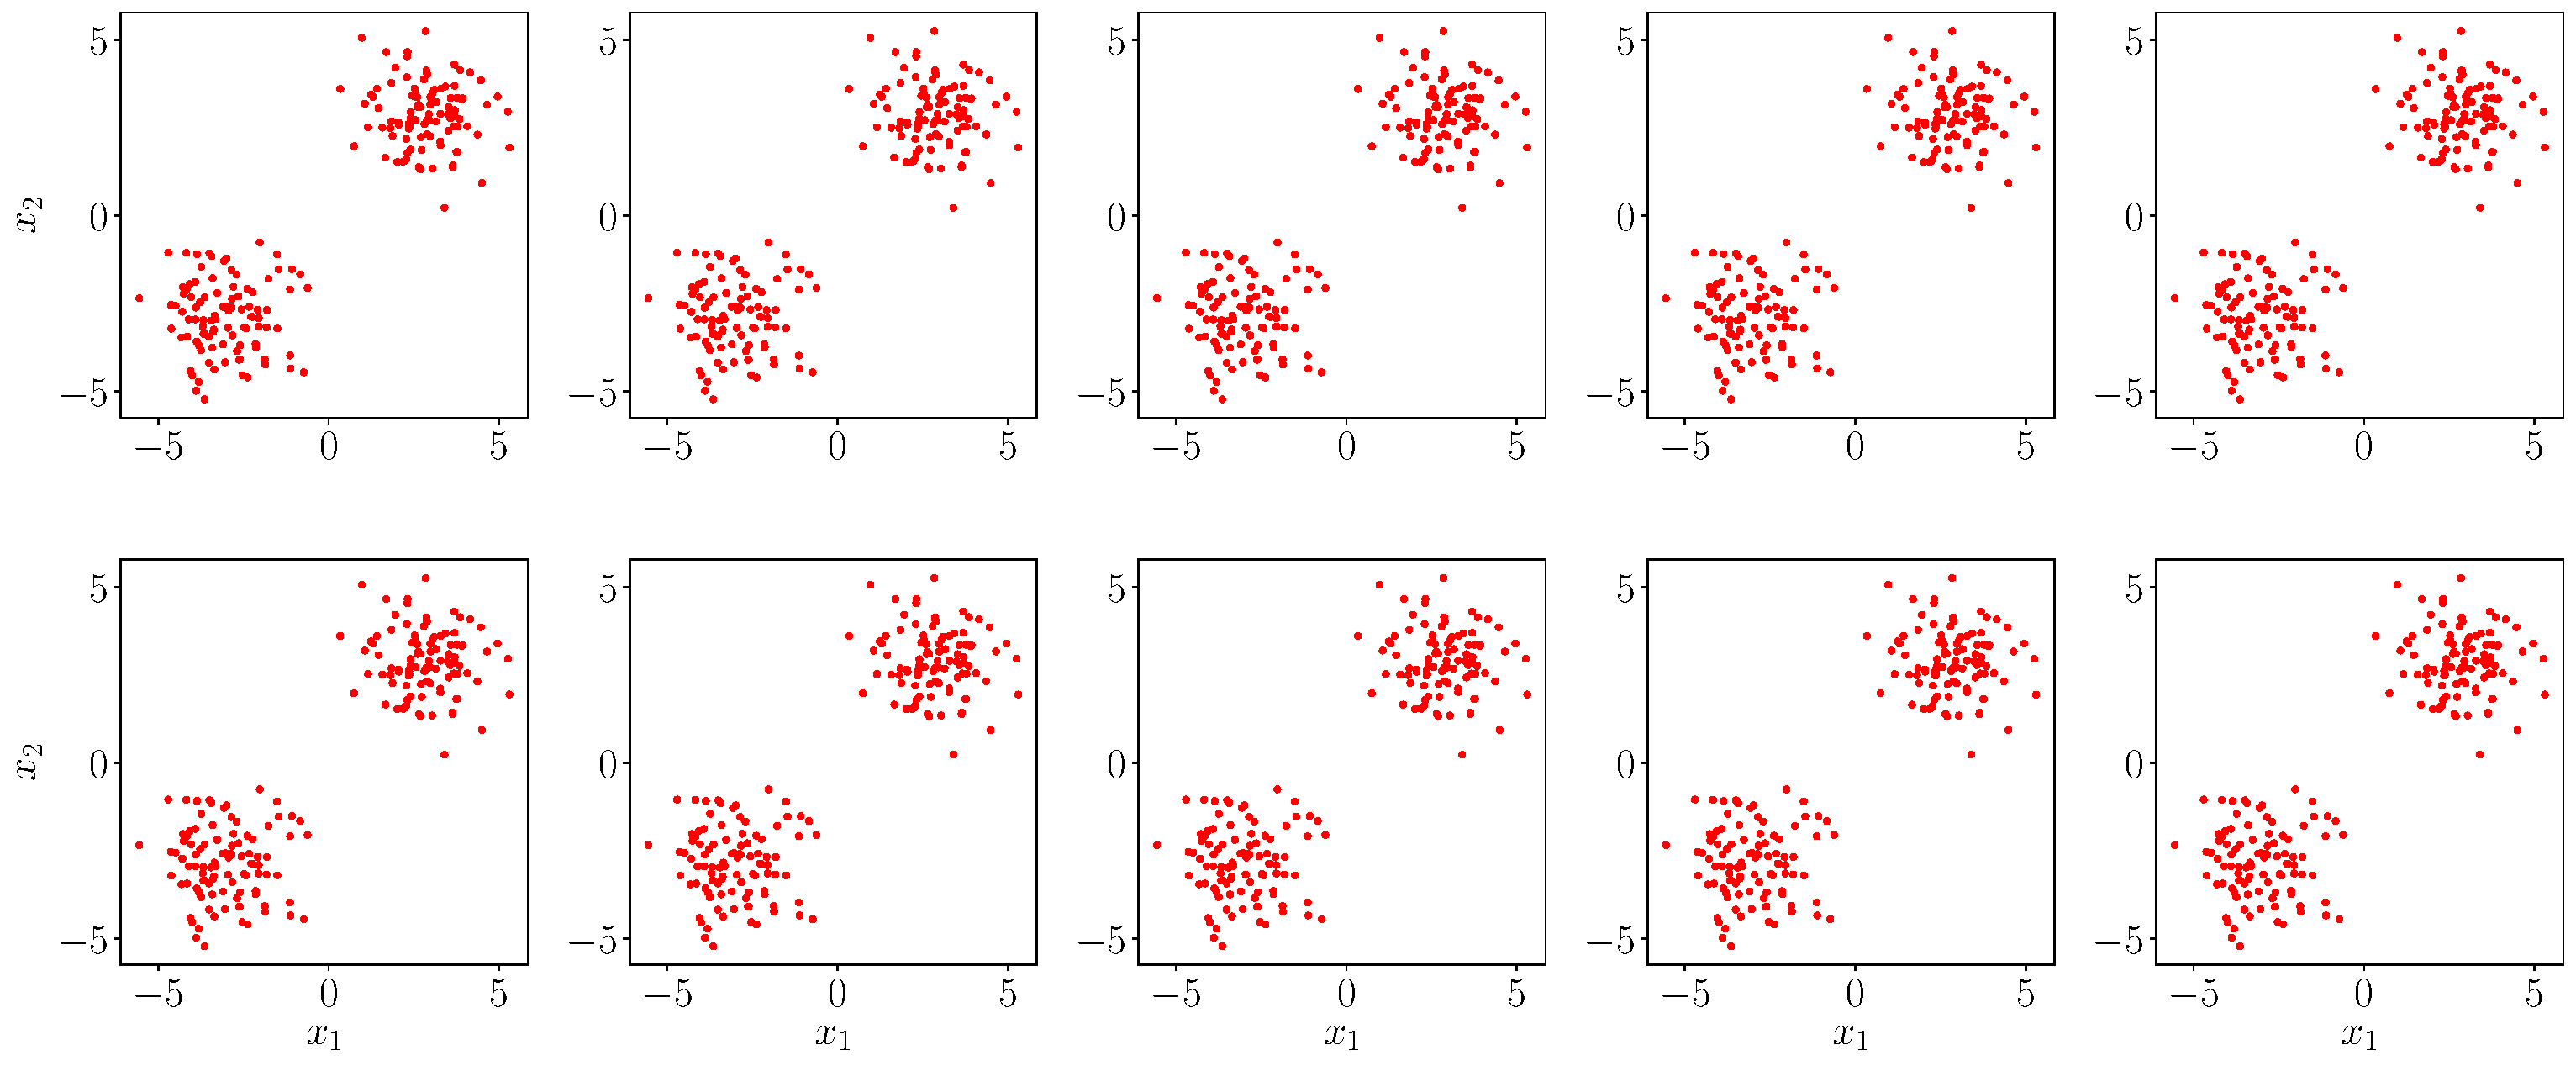
\includegraphics[height=0.35\textheight]{pictures/pi_predicftion_models}\label{sl:8:pic:1}}
	\subfloat[]{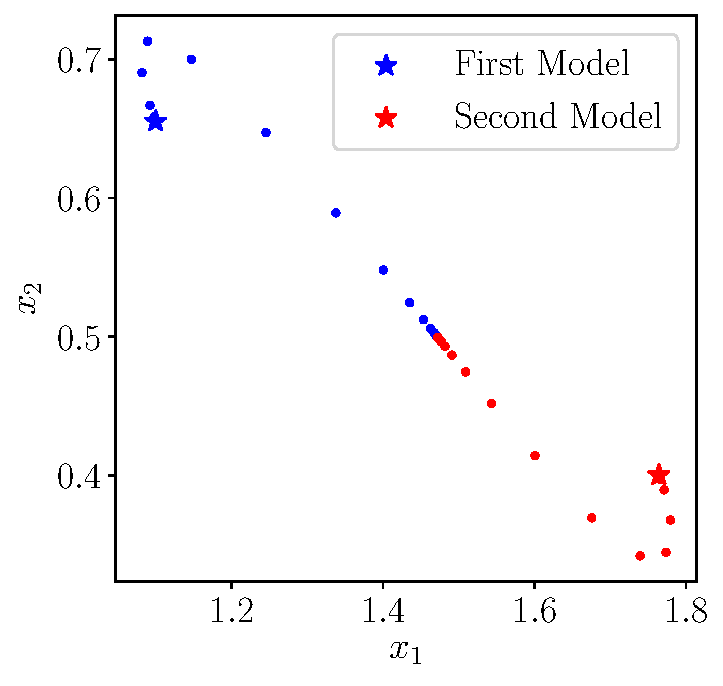
\includegraphics[height=0.35\textheight]{pictures/parameters_models}\label{sl:8:pic:2}}
\end{figure}
На рис.~\ref{sl:8:pic:1} показано, что в случае смеси моделей, предсказать то, какую модель использовать в каждой точке нельзя.

На рис.~\ref{sl:8:pic:2} показана зависимость векторов $\mathbf{w}_{k}$~---~параметры локальных моделей в процессе обучения.

\footnotetext[1]{\url{https://github.com/andriygav/MixtureLib}}
\end{frame}
%----------------------------------------------------------------------------------------------------------
\begin{frame}{Смесь экспертов}
\justifying
\begin{definition}
\label{sl:5:eq:1}
Смесь экспертов~---~мультимодель, определяющая правдоподобие веса $\pi_k$ каждой локальной модели $\textbf{f}_k$ на признаковом описании объекта $\textbf{x}$.

\begin{equation}
\label{sl:5:eq:2}
\begin{aligned}
\hat{\mathbf{f}} = \sum_{k=1}^{K}\pi_{k}\mathbf{f}_k, \qquad \pi_{k}\left(\mathbf{x}, \mathbf{V}\right):\mathbb{R}^{n\times \left|\mathbf{V}\right|} \to [0, 1], \qquad \sum_{k=1}^{K}\pi_{k}\left(\mathbf{x}, \mathbf{V}\right) = 1
\end{aligned}
\end{equation}
где~$\hat{\mathbf{f}}$~---~мультимодель, а $\mathbf{f}_k$ является некоторой моделью, $\pi_k$~---~параметрическая модель, $\mathbf{w}_k$~---~параметры $k$-й локальной модели, $\mathbf{V}$~---~параметры шлюзовой функции.
\end{definition}
{\bf Пример 2}:
	\begin{enumerate}
		\item Правдоподобие $k$-й локальной модели $p_{k}\left(y_{i}|\mathbf{w}_{k}, \mathbf{x}_{i}\right) = \mathcal{N}\left(y_{i}|\mathbf{w}_{k}^{\mathsf{T}}\mathbf{x}_{i}, \beta^{-1}\right),$
		\item Априорное распределение параметров $k$-й локальной модели $p^{k}\left(\mathbf{w}_{k}\right) = \mathcal{N}\left(\mathbf{w}_{k}|\mathbf{w}^{0}_{k}, \mathbf{A}_{k}\right),$
		\item Шлюзовая функция $\bm{\pi}\left(\mathbf{x}, \mathbf{V}\right) = \text{softmax}\bigr(\mathbf{V}_{1}^{\mathsf{T}}\bm{\sigma}\left(\mathbf{V}_2^{\mathsf{T}}\mathbf{x}\right)\bigr).$
	\end{enumerate}
\end{frame}
%----------------------------------------------------------------------------------------------------------
\begin{frame}{Пример 2}
\justifying
Правдоподобие модели:
	\begin{equation}
	\label{sl:6:eq:1}
		\begin{aligned}
			p\bigr(\mathbf{y}, \mathbf{W}|\mathbf{X}, \mathbf{V}, \textbf{A}, \textbf{W}^{0}, \beta\bigr) = \prod_{k=1}^{K}\mathcal{N}\left(\mathbf{w}_{k}|\mathbf{w}^{0}_{k}, \mathbf{A}_{k}\right)\prod_{i=1}^{N}\left(\sum_{k=1}^{K}\pi_{k}\mathcal{N}\left(y_{i}|\mathbf{w}_{k}^{\mathsf{T}}\mathbf{x}_{i}, \beta^{-1}\right)\right).
		\end{aligned}
	\end{equation}
Введем скрытые переменные $\textbf{Z} = ||z_{ik}||,$ где $~z_{ik} = 1 \Leftrightarrow k_i=k$:
	\begin{equation}
	\label{sl:6:eq:2}
		\begin{aligned}
			p\bigr(\mathbf{y}, \textbf{Z}, \mathbf{W}|\mathbf{X}, \mathbf{V}, \textbf{A}, \textbf{W}^{0}, \beta\bigr) = \prod_{k=1}^{K}\mathcal{N}\left(\mathbf{w}_{k}|\mathbf{w}^{0}_{k}, \mathbf{A}_{k}\right)\prod_{i=1}^{N}\prod_{k=1}^{K}\left(\pi_{k}\mathcal{N}\left(y_{i}|\mathbf{w}_{k}^{\mathsf{T}}\mathbf{x}_{i}, \beta^{-1}\right)\right)^{z_{ik}}.		
		\end{aligned}
	\end{equation}
Вариационный ЕМ--алгоритм $q\left(\textbf{Z}, \textbf{W}\right) = q\left(\textbf{Z}\right)q\left(\textbf{W}\right)$:
	\begin{enumerate}
		\item Е--шаг: 
			\begin{equation}
			\label{sl:6:eq:3}
				\begin{aligned}
					\log q\left(\textbf{Z}^{s}\right) &\propto \mathsf{E}_{q/\textbf{Z}}\log p\bigr(\mathbf{y}, \textbf{Z},\mathbf{W}|\mathbf{X}, \mathbf{V}^{s-1}, \textbf{A}^{s-1}, \textbf{W}^{0, s-1}, \beta^{s-1}\bigr)\\
					\log q\left(\textbf{W}^{s}\right) &\propto \mathsf{E}_{q/\textbf{W}}\log p\bigr(\mathbf{y}, \textbf{Z},\mathbf{W}|\mathbf{X}, \mathbf{V}^{s-1}, \textbf{A}^{s-1}, \textbf{W}^{0, s-1}, \beta^{s-1}\bigr)
				\end{aligned}
			\end{equation}
		\item М--шаг: 
			\begin{equation}
			\label{sl:6:eq:4}
				\begin{aligned}
					\textbf{W}^{0, s}, \textbf{A}^{s}, \beta^{s} = \arg\max_{\textbf{W}^{0}, \textbf{A}, \beta} \mathbf{E}_{q^{s}}\log p\bigr(\mathbf{y}, \textbf{Z},\mathbf{W}|\mathbf{X}, \mathbf{V}, \textbf{A}, \textbf{W}^{0}, \beta\bigr)
				\end{aligned}
			\end{equation}
	\end{enumerate}
\end{frame}
%----------------------------------------------------------------------------------------------------------
\begin{frame}{Пример 2}
\justifying
Итерационные формулы ЕМ--алгоритма\footnote[1]{\url{https://github.com/andriygav/EMprior/blob/master/paper/Grabovoy2019MixtureOfExpert.pdf}}:
	\begin{enumerate}
		\item Е--шаг: 
			\begin{equation}
			\label{sl:7:eq:1}
				\begin{aligned}
					&p\left(z_{ik} = 1\right) = \frac{\exp\left(\log\pi_{k}\left(\textbf{x}_{i}, \textbf{V}\right) - \frac{\beta}{2}\left(\textbf{x}_{i}^{\mathsf{T}}\mathsf{E}\textbf{w}_{k}\textbf{w}_{k}^{\mathsf{T}}\textbf{x}_{i} - \textbf{x}_{i}^{\mathsf{T}}\mathsf{E}\textbf{w}_{k}\right)\right)}{\sum_{k'=1}^{K}\exp\left(\log\pi_{k'}\left(\textbf{x}_{i}, \textbf{V}\right) - \frac{\beta}{2}\left(\textbf{x}_{i}^{\mathsf{T}}\mathsf{E}\textbf{w}_{k'}\textbf{w}_{k'}^{\mathsf{T}}\textbf{x}_{i} - \textbf{x}_{i}^{\mathsf{T}}\mathsf{E}\textbf{w}_{k'}\right) \right)},\\
					&q(\textbf{w}_k) = \mathcal{N}(\textbf{w}_k|\textbf{m}_k, \textbf{B}_k),\\
					&\mathbf{m}_{k} = \mathbf{B}_{k}\left(\mathbf{A}_{k}^{-1}\mathbf{w}_{k}^{0}+\beta\sum_{i=1}^{N}\mathbf{x}_{i}y_{i}\mathsf{E}z_{ik}\right), \quad
					\mathbf{B}_{k} = \left(\mathbf{A}_{k}^{-1}+\beta\sum_{i=1}^{N}\mathbf{x}_{i}\mathbf{x}_{i}^{\mathsf{T}}\mathsf{E}z_{ik}\right)^{-1} .
				\end{aligned}
			\end{equation}
		\item М--шаг: 
			\begin{equation}
			\label{sl:7:eq:2}
				\begin{aligned}
					&\textbf{A}_{k} = \mathsf{E}\textbf{w}_{k}\textbf{w}_{k}^{\mathsf{T}} - \textbf{w}_{k}^{0}\mathsf{E}\textbf{w}_{k}^{\mathsf{T}} - \mathsf{E}\textbf{w}_{k}\textbf{w}_{k}^{0\mathsf{T}} + \textbf{w}_{k}^{0}\textbf{w}_{k}^{0\mathsf{T}}, \\
					 &\frac{1}{\beta}=\frac{1}{N}\sum_{i=1}^{N}\sum_{k=1}^{K}\left[y_{i}^{2}-2y_{i}\textbf{x}_{i}^{\mathsf{T}}\mathsf{E}\textbf{w}_{k} + \textbf{x}_{i}^{\mathsf{T}}\mathsf{E}\textbf{w}_{k}\textbf{w}_{k}^{\mathsf{T}}\textbf{x}_{i}\right]\mathsf{E}z_{ik},\\
					&\textbf{w}_{k}^{0} =\mathsf{E}\textbf{w}_{k},\\
					&\textbf{V}= \arg\max_{\textbf{V}} \mathbf{E}_{q^{s}}\log p\bigr(\mathbf{y}, \textbf{Z},\mathbf{W}|\mathbf{X}, \mathbf{V}, \textbf{A}, \textbf{W}^{0}, \beta\bigr).
				\end{aligned}
			\end{equation}
	\end{enumerate}
\end{frame}
%----------------------------------------------------------------------------------------------------------
\begin{frame}{Пример 2}
\justifying
\begin{figure}
	\subfloat[]{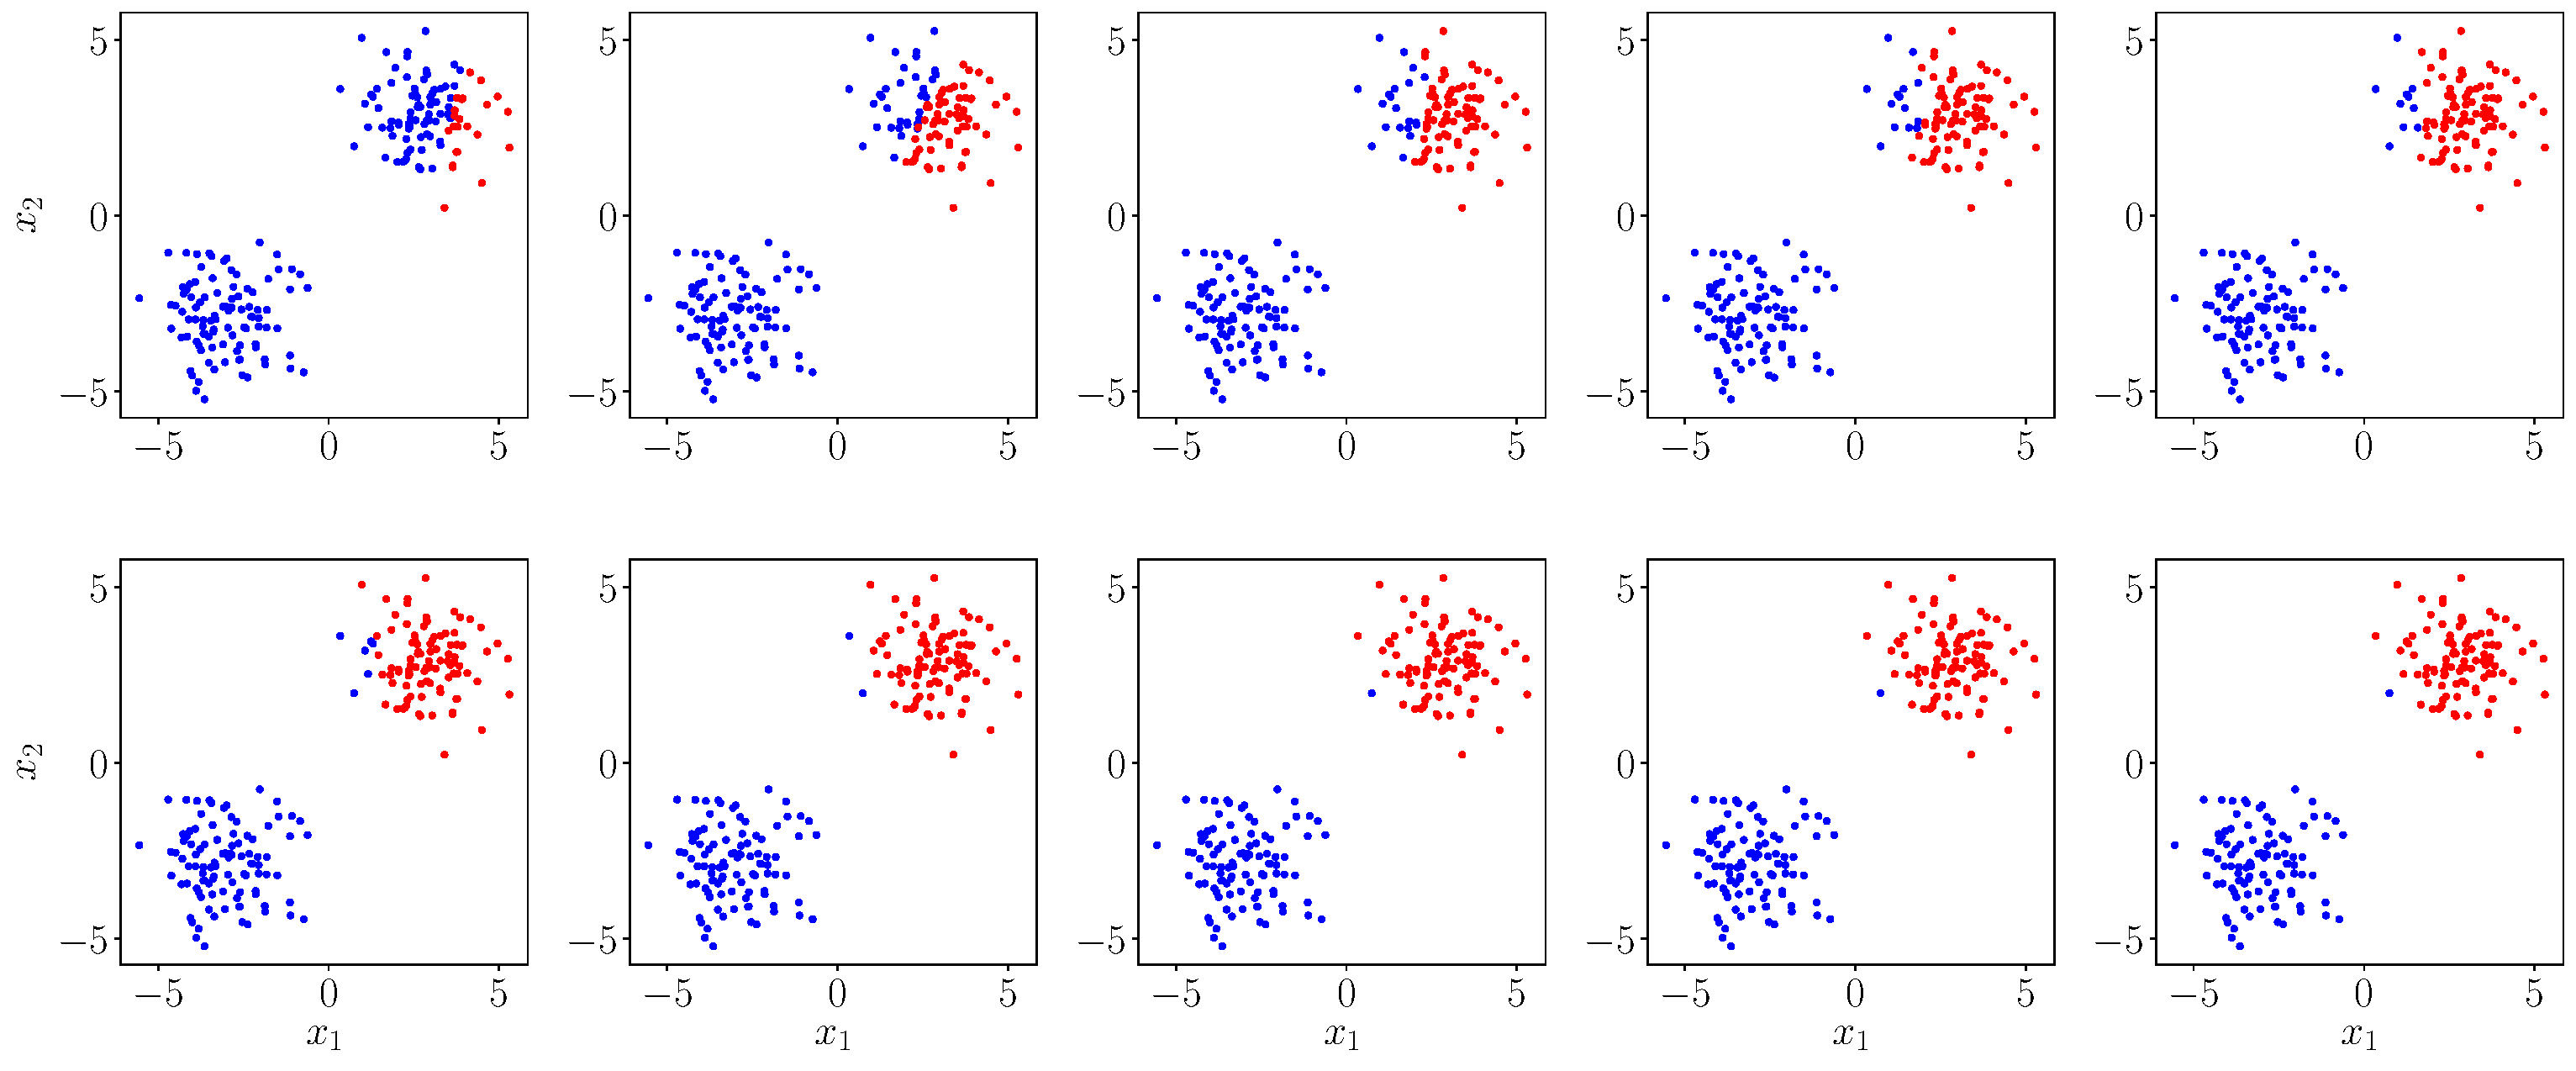
\includegraphics[height=0.35\textheight]{pictures/pi_predicftion_experts}\label{sl:9:pic:1}}
	\subfloat[]{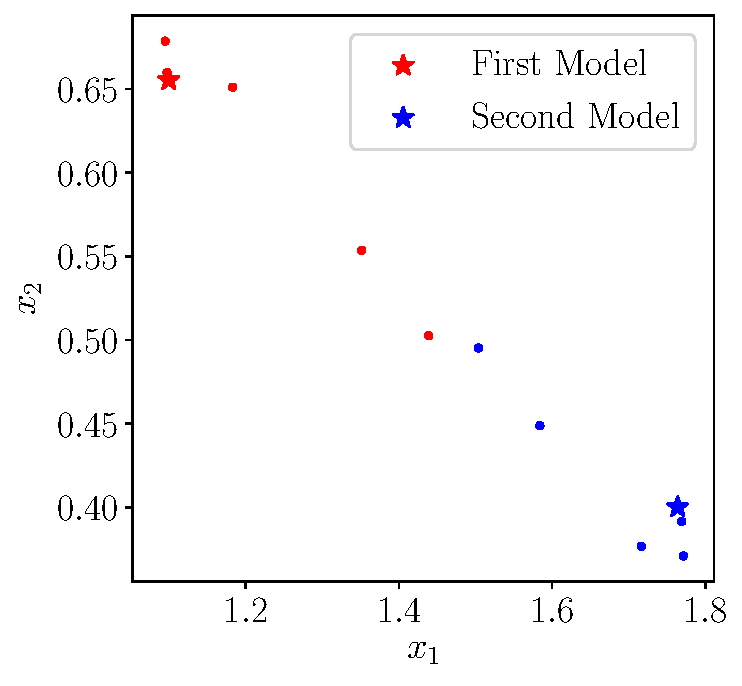
\includegraphics[height=0.35\textheight]{pictures/parameters_experts}\label{sl:9:pic:2}}
\end{figure}
На рис.~\ref{sl:9:pic:1} показано, что в случае смеси экспертов гипермодель предсказывает к какому классу относится каждая точка в пространстве объектов.

На рис.~\ref{sl:9:pic:2} показана зависимость векторов $\mathbf{w}_{k}$~---~параметры локальных моделей в процессе обучения.

\footnotetext[1]{\url{https://github.com/andriygav/MixtureLib}}
\end{frame}
%----------------------------------------------------------------------------------------------------------
\begin{frame}{Сравнение результатов}
\justifying
\begin{figure}
	\subfloat[Смесь Моделей]{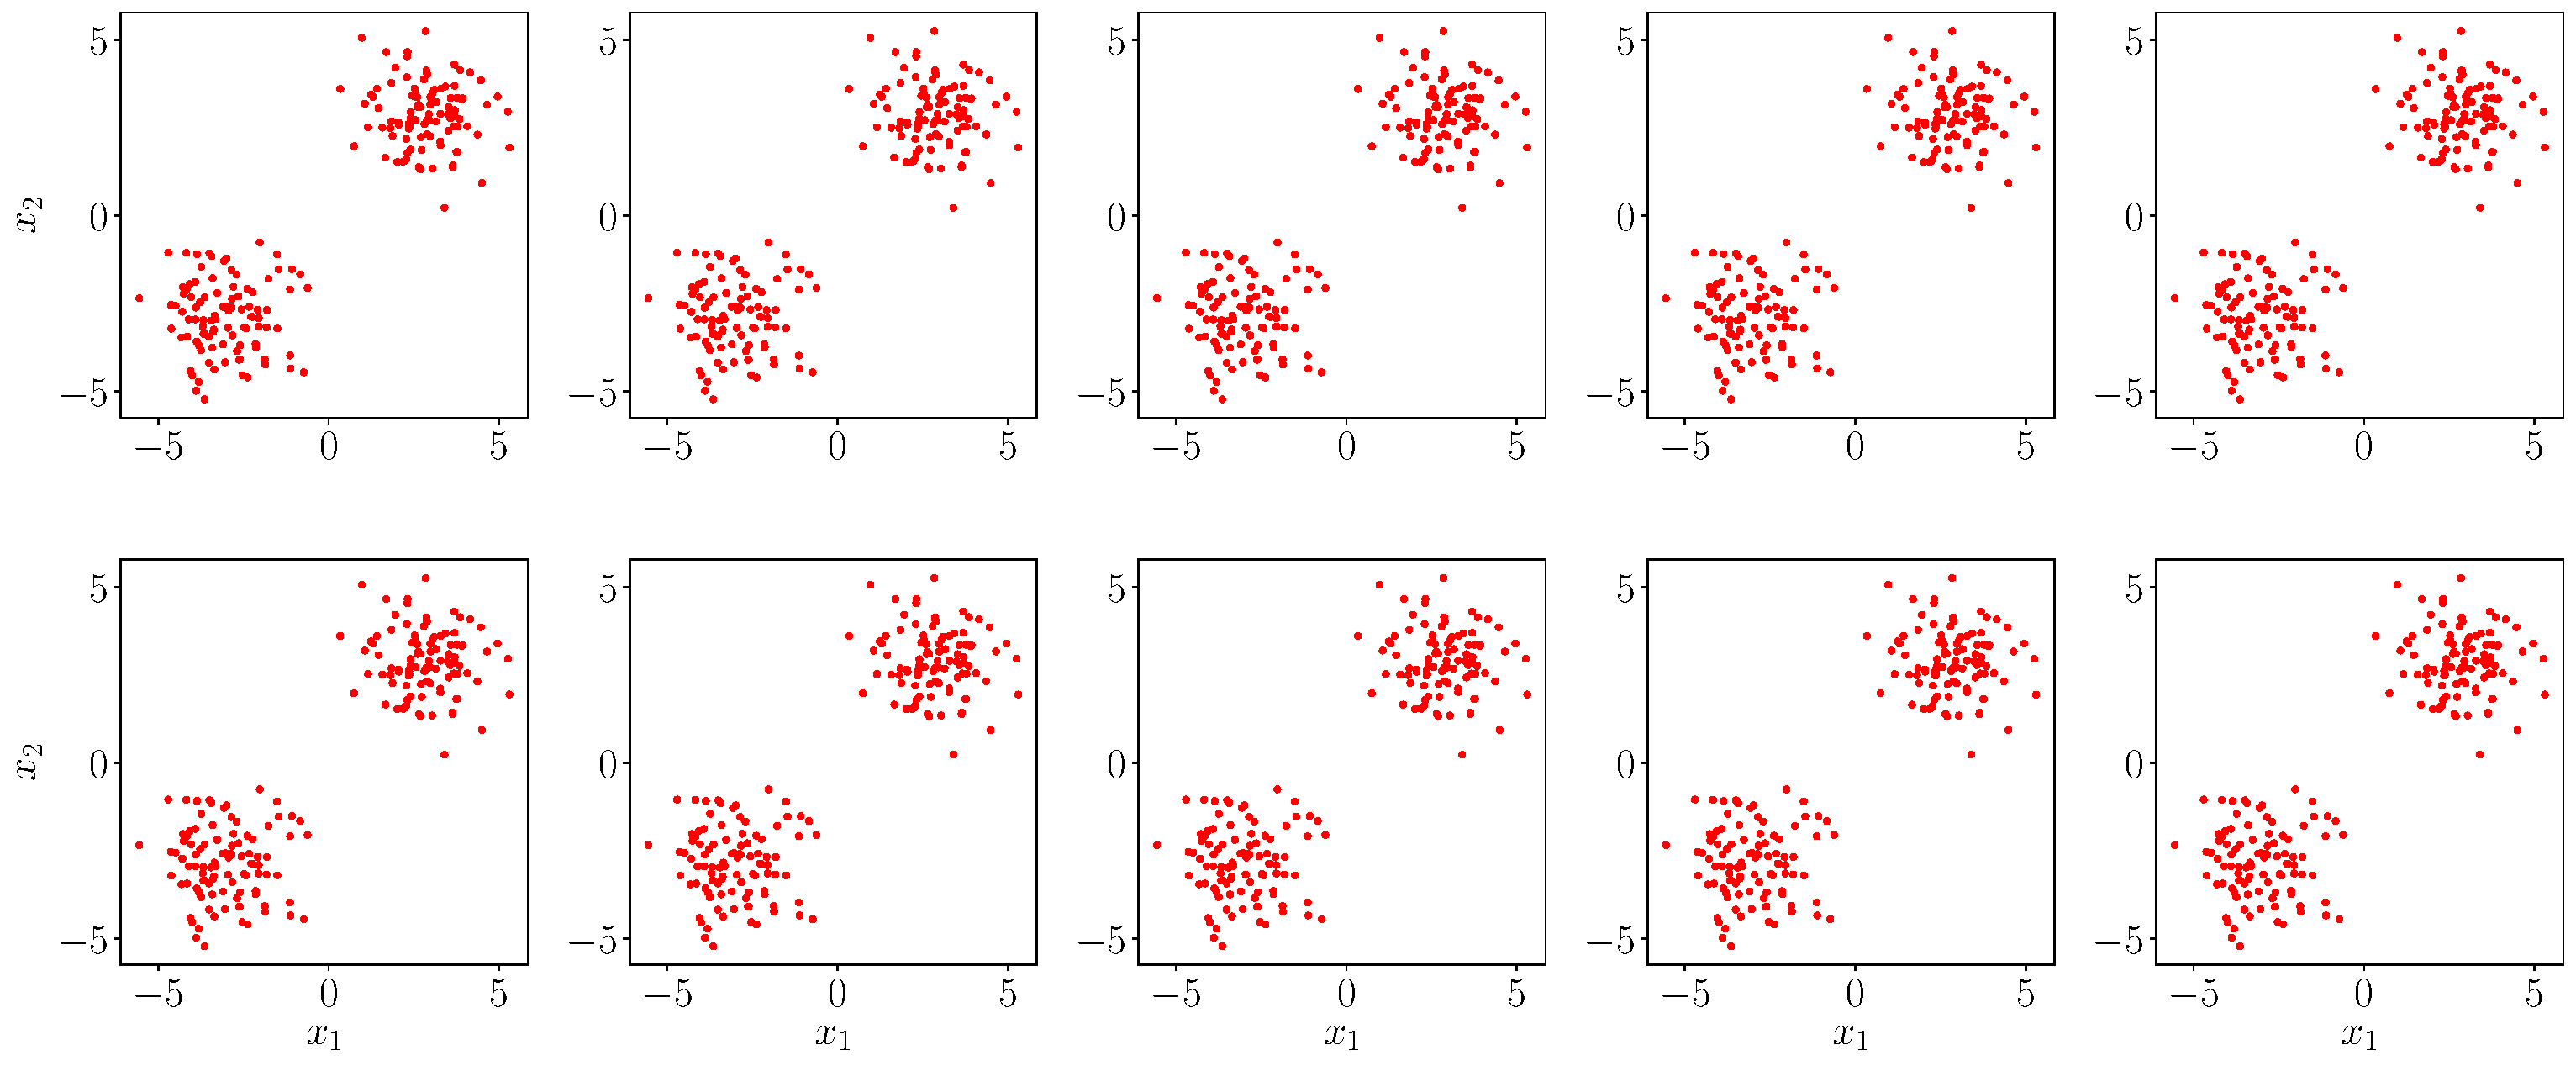
\includegraphics[height=0.35\textheight]{pictures/pi_predicftion_models}\label{sl:10:pic:1}}
	\subfloat[Смесь Моделей]{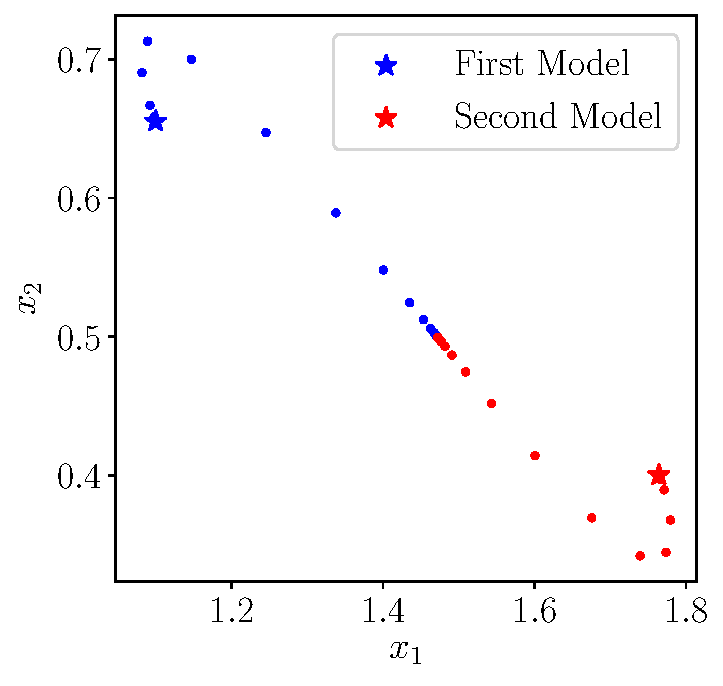
\includegraphics[height=0.35\textheight]{pictures/parameters_models}\label{sl:10:pic:2}}\\
	\subfloat[Смесь Экспертов]{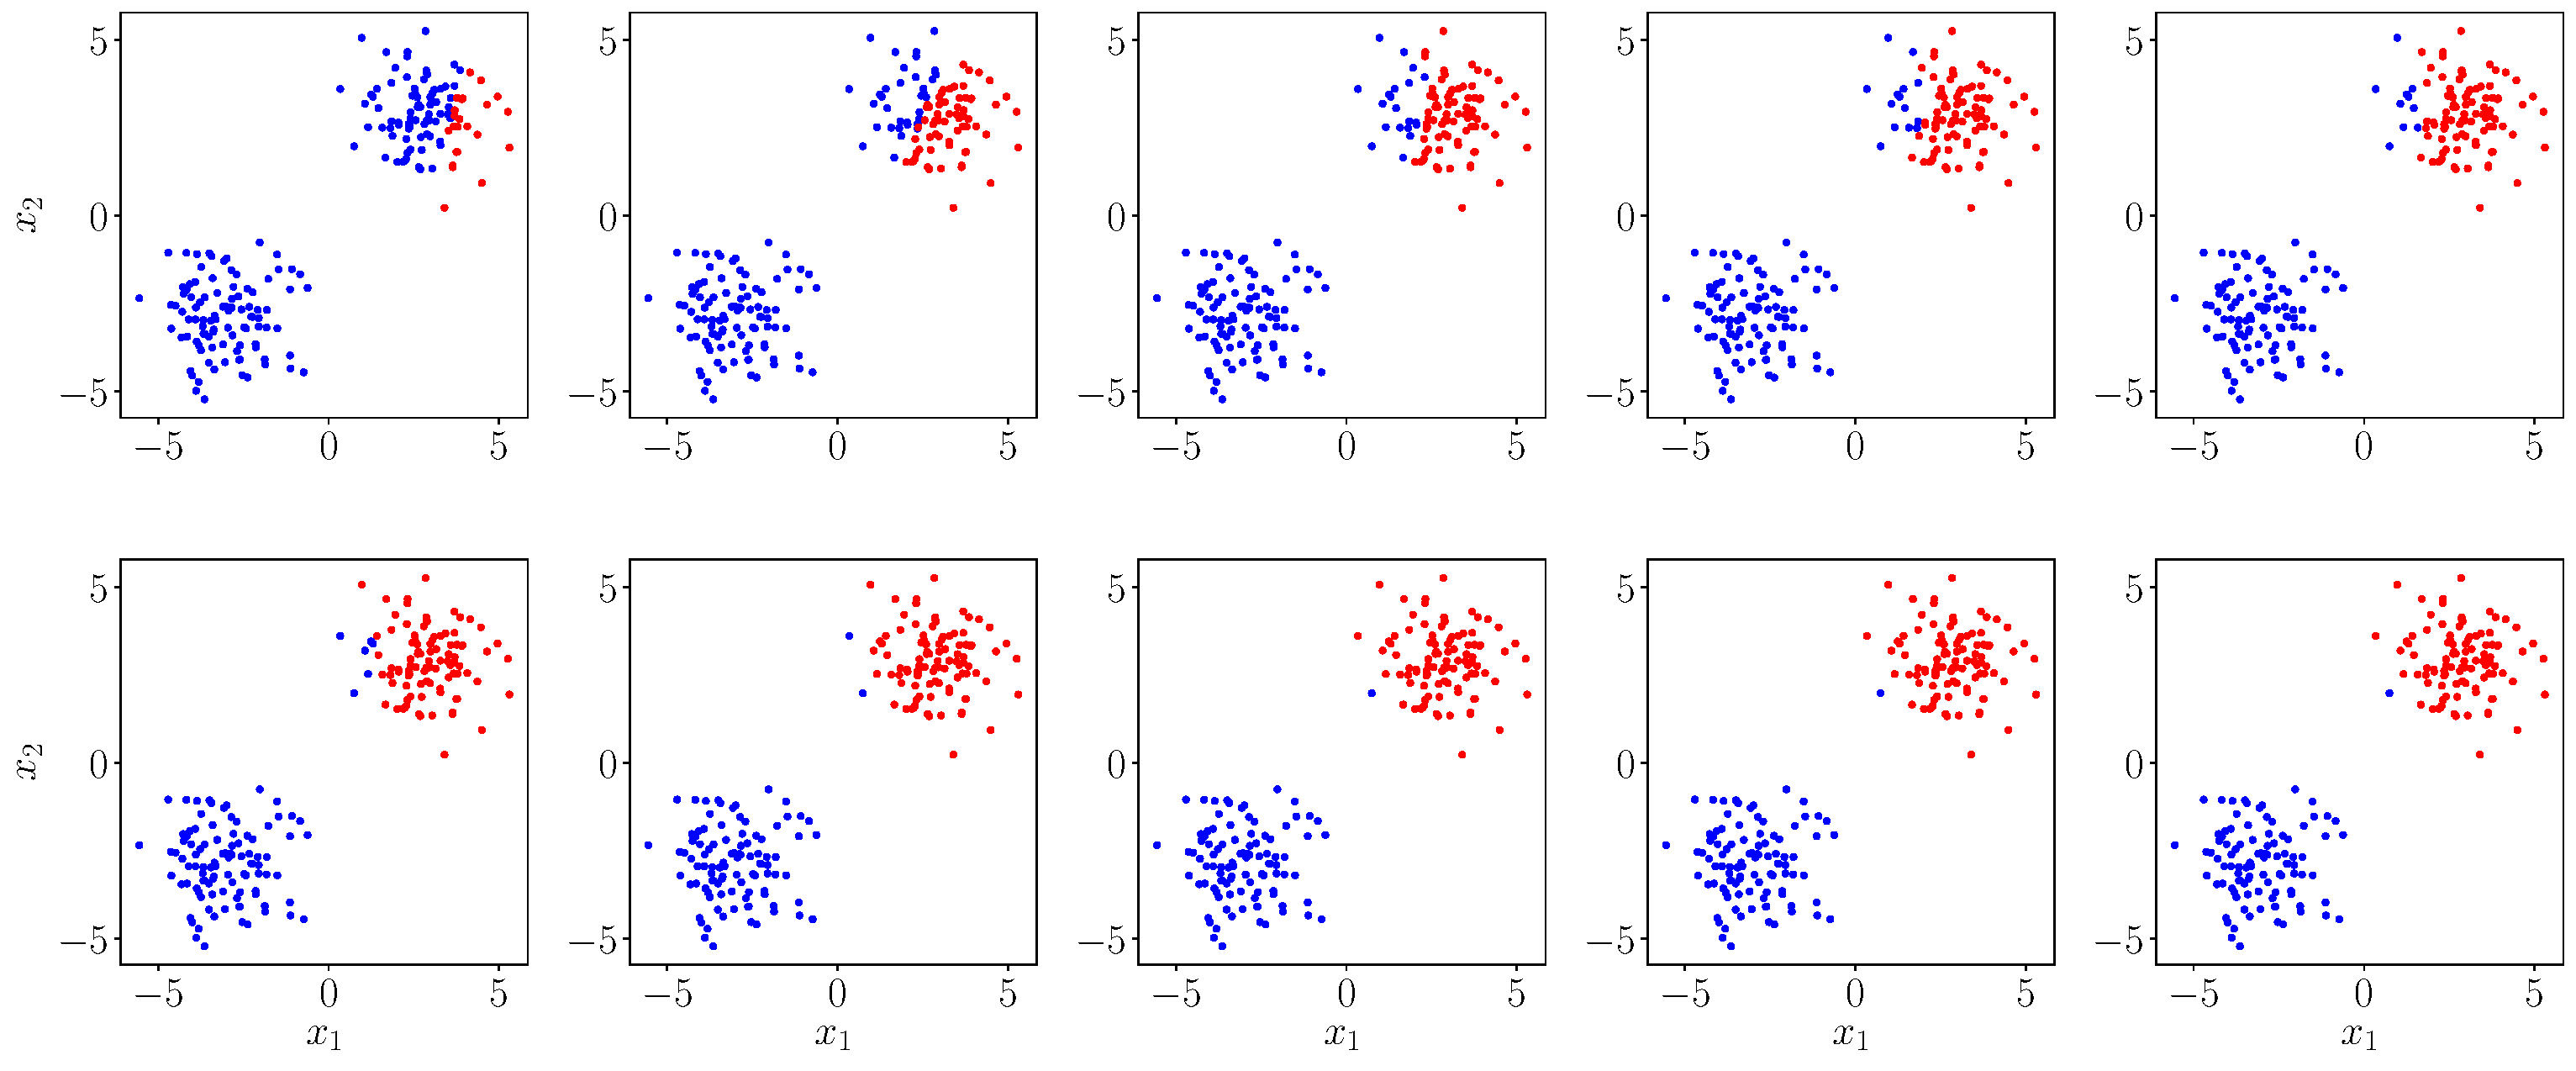
\includegraphics[height=0.35\textheight]{pictures/pi_predicftion_experts}\label{sl:10:pic:3}}
	\subfloat[Смесь Экспертов]{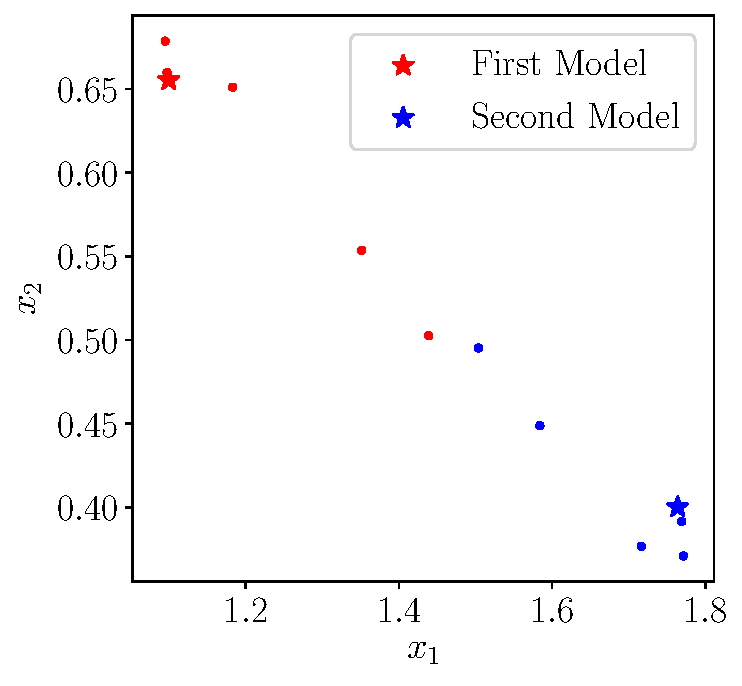
\includegraphics[height=0.35\textheight]{pictures/parameters_experts}\label{sl:10:pic:4}}
\end{figure}
\footnotetext[1]{\url{https://github.com/andriygav/MixtureLib}}
\end{frame}
%----------------------------------------------------------------------------------------------------------


%----------------------------------------------------------------------------------------------------------
\begin{frame}{Построение ансамбля локальных моделей}
\justifying
\textbf{Цель:} предложить метод построения ансамбля локально аппроксимирующих моделей для поиска окружностей на изображении.

~\\
\textbf{Задачи}

\begin{enumerate}
\justifying
	\item Предложить метод поиска окружности при помощи линейной модели, для поиска нескольких окружностей предложить метод построения смеси локальных аппроксимирующих моделей.
	\item Предложить априорные распределения на параметры локальных моделей.
\end{enumerate}

~\\
\textbf{Исследуемая проблема}
\begin{enumerate}
\justifying
	\item Снижение размерности пространства описаний изображения.
\end{enumerate}

~\\
\textbf{Метод решения}

	В качестве мультимодели предлагается использовать смесь экспертов. Для повышения качества мультимодели предлагается ввести априорные распределения параметров локальных моделей. Вводится \textit{регуляризация} априорных распределений для учета взаимосвязи между априорными распределениями разных локальных моделей смеси.
	
\end{frame}
%----------------------------------------------------------------------------------------------------------
\begin{frame}{Список литературы}
	\begin{enumerate}
	\justifying
		\item \textit{Yuksel Seniha Esen, Wilson Joseph N., Gader Paul D} Twenty Years of Mixture of Experts~// IEEE Transactions on Neural Networks and Learning Systems. 2012. Issues. 23, No 8. pp. 1177--1193.
		\item \textit{A. P. Dempster, N. M. Laird and D. B. Rubin} Maximum Likelihood from Incomplete Data via the EM Algorithm~// Journal of the Royal Statistical Society. Series B (Methodological), Vol. 39, No. 1 pp. 1-38, 1977.
		\item \textit{Bishop C.} Pattern Recognition and Machine Learning.~---~Berlin: Springer, 2006. 758~p.
		\item \textit{I. Matveev} Detection of iris in image by interrelated maxima of brightness gradient projections~// Appl.Comput. Math. 9 (2), 252–257, 2010.
		\item \textit{K. Bowyer, K. Hollingsworth, P. Flynn} A Survey of Iris Biometrics Research: 2008–2010.
		
	\end{enumerate}
\end{frame}

%----------------------------------------------------------------------------------------------------------
\begin{frame}[shrink=5]{Постановка задачи нахождения параметров окружностей}
\justifying
\begin{columns}
\column{0.6\textwidth}
Задано бинарное изображение:
\begin{equation*}
\begin{aligned}
\textbf{M} \in \{0,1\}^{m_1 \times m_2},
\end{aligned}
\end{equation*}
где $1$ --- черная точка, $0$ --- белая точка фона.

По изображению $\textbf{M}$ строится выборка $\textbf{C}$:
\begin{equation*}
\begin{aligned}
\textbf{C} \in  \mathbb{R}^{N \times 2},
\end{aligned}
\end{equation*}
где $N$ --- число черных точек на изображении $\textbf{M}$.
\column{0.36\textwidth}
\begin{center}
	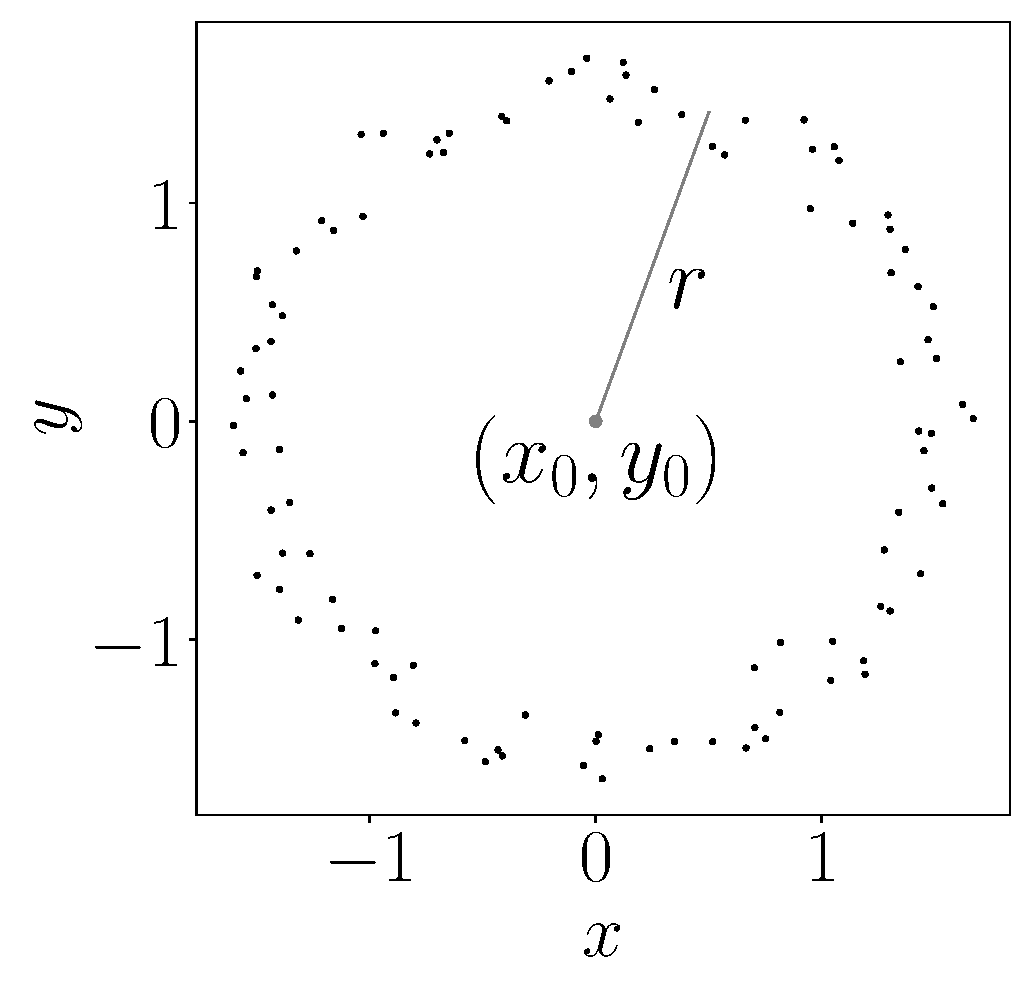
\includegraphics[height=0.4\textheight]{result/slides_statment}
\end{center}
\end{columns}


Пусть $x_0, y_0$~--- центр окружности, которую требуется найти, а $r$ ее радиус.

Точки~$\left(x_i, y_i\right)\in\textbf{C}$ должны удовлетворять уравнению окружности:
\begin{equation*}
\begin{aligned}
\left(x_i - x_0\right)^{2}+\left(y_i-y_0\right)^2 = r^2 \Rightarrow (2x_0)\cdot x_i + (2y_0)\cdot y_i+(r^2-x_0^2-y_0^2)\cdot1 = x_{i}^2 + y_{i}^2.
\end{aligned}
\end{equation*}
Задачу линейной регрессии для нахождения окружности:
\begin{equation*}
\begin{aligned}
\textbf{X}\textbf{w} \approx \textbf{y},  \quad \textbf{X} = \left[\textbf{C}, \textbf{1}\right], \quad \textbf{y} = [x_1^2+y_1^2, x_2^2+y_2^2, \cdots, x_N^2+y_N^2]^{\mathsf{T}},
\end{aligned}
\end{equation*}
где найденые оптимальные параметры линейной регрессии $\textbf{w} = \bigr[w_1, w_2, w_3\bigr]^{\mathsf{T}}$ восстанавливают параметры окружности:
\begin{equation*}
\begin{aligned}
x_0 = \frac{w_1}{2}, \quad y_0 = \frac{w_2}{2}, \quad r = \sqrt[]{w_3+x_{0}^{2}+y_{0}^{2}}.
\end{aligned}
\end{equation*}

\end{frame}
%----------------------------------------------------------------------------------------------------------
\begin{frame}{Универсальная модель--ансамбль: смесь экспертов}
\justifying
Задана выборка:
\begin{equation*}
\begin{aligned}
\textbf{X} \in \mathbb{R}^{N \times n},
\end{aligned}
\end{equation*}
где~$N$~---~число объектов в выборке, а~$n$~---~размерность признакового пространства.


\begin{definition}
Смесь экспертов~---~мультимодель, определяющая правдоподобие веса $\pi_k$ каждой локальной модели $\textbf{f}_k$ на признаковом описании объекта $\textbf{x}$.
\begin{equation*}
\begin{aligned}
\hat{\mathbf{f}} = \sum_{k=1}^{K}\pi_{k}\mathbf{f}_k, \qquad \pi_{k}\left(\mathbf{x}, \mathbf{V}\right):\mathbb{R}^{n\times \left|\mathbf{V}\right|} \to [0, 1], \qquad \sum_{k=1}^{K}\pi_{k}\left(\mathbf{x}, \mathbf{V}\right) = 1,
\end{aligned}
\end{equation*}
где~$\hat{\mathbf{f}}$~---~мультимодель, а $\mathbf{f}_k$ является локальной моделью, $\pi_k$~---~шлюзовая функция, $\mathbf{w}_k$~---~параметры $k$-й локальной модели, $\mathbf{V}$~---~параметры шлюзовой функции.
\end{definition}

В качестве локальных моделей~$\mathbf{f}_k$ и шлюзовой функции~$\bm{\pi}$ рассматриваются следующие функции:
\begin{equation*}
\begin{aligned}
\mathbf{f}_k\left(\textbf{x}\right) = \textbf{w}_k^{\mathsf{T}}\textbf{x}, \quad
\bm{\pi}\left(\mathbf{x}, \mathbf{V}\right) = \text{softmax}\bigr(\mathbf{V}_{1}^{\mathsf{T}}\bm{\sigma}\bigr(\mathbf{V}_2^{\mathsf{T}}\mathbf{x}\bigr)\bigr),
\end{aligned}
\end{equation*}
где $\mathbf{V} = \bigr\{\mathbf{V}_1, \mathbf{V}_2\bigr\}$~---~параметры шлюзовой функции.


\end{frame}
%----------------------------------------------------------------------------------------------------------
\begin{frame}{Оптимизация параметров}
\justifying
Параметры локальных моделей оптимизируются согласно принципу максимального правдоподобия модели:
\begin{equation*}
\begin{aligned}
p\bigr(\mathbf{y}, \mathbf{W}|\mathbf{X}, \mathbf{V}\bigr) = \prod_{k=1}^{K}p^{k}\bigr(\mathbf{w}_k\bigr)\prod_{i=1}^{N}\left(\sum_{k=1}^{K}\pi_{k}p_{k}\bigr(y_i|\mathbf{w}_k, \mathbf{x}_i\bigr)\right),
\end{aligned}
\end{equation*}
где $\mathbf{W} = \bigr[\mathbf{w}_1, \mathbf{w}_2, \cdots, \mathbf{w}_K\bigr]^{\mathsf{T}}.$

Задача оптимизации параметров локальных моделей и параметров смеси:
\begin{equation*}
\begin{aligned}
\hat{\mathbf{W}}, \hat{\mathbf{V}} = \arg\max_{\mathbf{W}, \mathbf{V}} p\bigr(\mathbf{y}, \mathbf{W}|\mathbf{X}, \mathbf{V}\bigr).
\end{aligned}
\end{equation*}

Рассматривается вероятностная постановка задачи:
\begin{enumerate}
	\item[1)] правдоподобие выборки $p_{k}\left(y_{i}|\mathbf{w}_{k}, \mathbf{x}_{i}\right) = \mathcal{N}\left(y_{i}|\mathbf{w}_{k}^{\mathsf{T}}\mathbf{x}_{i}, \beta^{-1}\right),$ где $\beta$ уровень шума,
	\item[2)] априорное распределение параметров $p^{k}\left(\mathbf{w}_{k}\right) = \mathcal{N}\left(\mathbf{w}_{k}|\mathbf{w}^{0}_{k}, \mathbf{A}_{k}\right),$ где $\mathbf{w}^{0}_{k}$~---~вектор размера $n\times1,$ $\mathbf{A}_{k}$~---~ковариационная матрица параметров,
	\item[3)] регуляризация априорного распределения $p\left(\bm{\varepsilon}_{k,k'}|\bm{\alpha}\right) = \mathcal{N}\left(\bm{\varepsilon}_{k,k'}|\mathbf{0},  \bm{\Xi}\right),$ где~$\bm{\Xi}$~---~ковариационная матрица общего вида, $\bm{\varepsilon}_{k,k'} = \mathbf{w}_{k}^{0}-\mathbf{w}_{k'}^{0}.$
\end{enumerate}

\end{frame}
%----------------------------------------------------------------------------------------------------------
\begin{frame}{EM--алгоритм для решения задачи смеси экспертов}
\justifying
Правдоподобие модели включает правдоподобие выборки, априорное распределение параметров, а также их регуляризацию
\begin{equation*}
\begin{aligned}
p\bigr(\mathbf{y}, \mathbf{W}|\mathbf{X}, \mathbf{V}, \textbf{A}, \textbf{W}^{0}, \bm{\Xi}, \beta\bigr) = &\prod_{k,k'=1}^{K}\mathcal{N}\left(\bm{\varepsilon}_{k,k'}|\mathbf{0},  \bm{\Xi}\right)\cdot\\
&\cdot\prod_{k=1}^{K}\mathcal{N}\left(\mathbf{w}_{k}|\mathbf{w}^{0}_{k}, \mathbf{A}_{k}\right)\prod_{i=1}^{N}\left(\sum_{k=1}^{K}\pi_{k}\mathcal{N}\left(y_{i}|\mathbf{w}_{k}^{\mathsf{T}}\mathbf{x}_{i}, \beta^{-1}\right)\right),
\end{aligned}
\end{equation*}
где~$\mathbf{A} = \bigr\{\mathbf{A}_1, \cdots, \mathbf{A}_K\bigr\}.$
Введем скрытые переменные $\textbf{Z} = [z_{ik}],$ где $~z_{ik} = 1$ тогда и только тогда, когда $k_i=k$:
\begin{equation*}
\begin{aligned}
\log p\bigr(\mathbf{y}, \mathbf{Z}, \mathbf{W}&|\mathbf{X}, \mathbf{V}, \textbf{A}, \textbf{W}^{0},  \bm{\Xi}, \beta\bigr) =\\
&= \sum_{i=1}^{N}\sum_{k=1}^{K}z_{ik}\left[\log\pi_k\left(\textbf{x}_i, \textbf{V}\right) - \frac{\beta}{2}\left(y_{i} - \textbf{w}_{k}^{\mathsf{T}}\textbf{x}_{i}\right)^{2} + \frac{1}{2}\log\frac{\beta}{2\pi}\right] +\\
&+ \sum_{k=1}^{K}\left[-\frac{1}{2}\left(\textbf{w}_{k} - \textbf{w}_{k}^{0}\right)^{\mathsf{T}}\textbf{A}_{k}^{-1}\left(\textbf{w}_{k} - \textbf{w}_{k}^{0}\right) + \frac{1}{2}\log\det\textbf{A}^{-1}_{k} - \frac{n}{2}\log2\pi\right]+\\
&+ \sum_{k=1}^{K}\sum_{k'=1}^{K}\left[-\frac{1}{2}\left(\textbf{w}_{k}^{0}-\textbf{w}_{k'}^{0}\right)^{\mathsf{T}}\hat{\bm{\alpha}}^{-1}\left(\textbf{w}_{k}^{0}-\textbf{w}_{k'}^{0}\right) +\frac{1}{2}\log\det \bm{\Xi} -\frac{n}{2}\log{2\pi}\right].
\end{aligned}
\end{equation*}

\end{frame}
%----------------------------------------------------------------------------------------------------------
\begin{frame}{EM--алгоритм для решения задачи смеси экспертов}
\justifying
Задача оптимизации параметров локальных моделей и параметров смеси принимает следующий вид:
\begin{equation*}
\begin{aligned}
\mathbf{W}, \mathbf{Z}, \mathbf{V}, \mathbf{W}^0, \textbf{A},  \beta = \arg\max_{\mathbf{W}, \mathbf{Z}, \mathbf{V}, \mathbf{W}^0, \textbf{A}, \beta} \log p\bigr(\mathbf{y}, \mathbf{Z}, \mathbf{W}&|\mathbf{X}, \mathbf{V}, \textbf{A}, \textbf{W}^{0}, \bm{\Xi}, \beta\bigr).
\end{aligned}
\end{equation*}

Для оптимизации используется вариационный ЕМ--алгоритм с аппроксимацией среднего поля~$q\left(\textbf{Z}, \textbf{W}\right) = q\left(\textbf{Z}\right)q\left(\textbf{W}\right)$.

Е и М шаги алгоритма имеют следующий вид:
	\begin{enumerate}
		\item Е--шаг: 
			\begin{equation*}
				\begin{aligned}
					\log q\left(\textbf{Z}^{s}\right) &\propto \mathsf{E}_{q/\textbf{Z}}\log p\bigr(\mathbf{y}, \textbf{Z},\mathbf{W}|\mathbf{X}, \mathbf{V}^{s-1}, \textbf{A}^{s-1}, \textbf{W}^{0, s-1}, \bm{\Xi}, \beta^{s-1}\bigr),\\
					\log q\left(\textbf{W}^{s}\right) &\propto \mathsf{E}_{q/\textbf{W}}\log p\bigr(\mathbf{y}, \textbf{Z},\mathbf{W}|\mathbf{X}, \mathbf{V}^{s-1}, \textbf{A}^{s-1}, \textbf{W}^{0, s-1}, \bm{\Xi}, \beta^{s-1}\bigr),
				\end{aligned}
			\end{equation*}
		\item М--шаг: 
			\begin{equation*}
				\begin{aligned}
					\textbf{W}^{0, s}, \textbf{A}^{s}, \textbf{V}^{s}, \beta^{s} = \arg\max_{\textbf{W}^{0}, \textbf{A}, \textbf{V}, \beta} \mathsf{E}_{q^{s}}\log p\bigr(\mathbf{y}, \textbf{Z},\mathbf{W}|\mathbf{X}, \mathbf{V}, \textbf{A}, \textbf{W}^{0}, \bm{\Xi}, \beta\bigr),
				\end{aligned}
			\end{equation*}
	\end{enumerate}
	где~$s$~--- номер итерации.
\end{frame}
%----------------------------------------------------------------------------------------------------------
\begin{frame}{EM--алгоритм для решения задачи смеси экспертов}
\justifying
Итерационные формулы ЕМ--алгоритма:
	\begin{enumerate}
		\item Е--шаг: 
			\begin{equation*}
				\begin{aligned}
					&p\left(z_{ik} = 1\right) = \frac{\exp\left(\log\pi_{k}\left(\textbf{x}_{i}, \textbf{V}\right) - \frac{\beta}{2}\left(\textbf{x}_{i}^{\mathsf{T}}\mathsf{E}\textbf{w}_{k}\textbf{w}_{k}^{\mathsf{T}}\textbf{x}_{i} - \textbf{x}_{i}^{\mathsf{T}}\mathsf{E}\textbf{w}_{k}\right)\right)}{\sum_{k'=1}^{K}\exp\left(\log\pi_{k'}\left(\textbf{x}_{i}, \textbf{V}\right) - \frac{\beta}{2}\left(\textbf{x}_{i}^{\mathsf{T}}\mathsf{E}\textbf{w}_{k'}\textbf{w}_{k'}^{\mathsf{T}}\textbf{x}_{i} - \textbf{x}_{i}^{\mathsf{T}}\mathsf{E}\textbf{w}_{k'}\right) \right)},\\
					&q(\textbf{w}_k) = \mathcal{N}(\textbf{w}_k|\textbf{m}_k, \textbf{B}_k),\\
					&\mathbf{m}_{k} = \mathbf{B}_{k}\left(\mathbf{A}_{k}^{-1}\mathbf{w}_{k}^{0}+\beta\sum_{i=1}^{N}\mathbf{x}_{i}y_{i}\mathsf{E}z_{ik}\right), \quad
					\mathbf{B}_{k} = \left(\mathbf{A}_{k}^{-1}+\beta\sum_{i=1}^{N}\mathbf{x}_{i}\mathbf{x}_{i}^{\mathsf{T}}\mathsf{E}z_{ik}\right)^{-1} .
				\end{aligned}
			\end{equation*}
		\item М--шаг: 
			\begin{equation*}
				\begin{aligned}
					&\textbf{A}_{k} = \mathsf{E}\textbf{w}_{k}\textbf{w}_{k}^{\mathsf{T}} - \textbf{w}_{k}^{0}\mathsf{E}\textbf{w}_{k}^{\mathsf{T}} - \mathsf{E}\textbf{w}_{k}\textbf{w}_{k}^{0\mathsf{T}} + \textbf{w}_{k}^{0}\textbf{w}_{k}^{0\mathsf{T}}, \\
					 &\frac{1}{\beta}=\frac{1}{N}\sum_{i=1}^{N}\sum_{k=1}^{K}\left[y_{i}^{2}-2y_{i}\textbf{x}_{i}^{\mathsf{T}}\mathsf{E}\textbf{w}_{k} + \textbf{x}_{i}^{\mathsf{T}}\mathsf{E}\textbf{w}_{k}\textbf{w}_{k}^{\mathsf{T}}\textbf{x}_{i}\right]\mathsf{E}z_{ik},\\
					&\textbf{w}_{k}^{0} =\left[\textbf{A}_{k}^{-1}+\left(K-1\right)\bm{\Xi}\right]^{-1}\left(\textbf{A}^{-1}_{k}\mathsf{E}\textbf{w}_{k}+\bm{\Xi}\sum_{k'=1,~k'\not=k}^{K}\textbf{w}_{k'}^{0}\right),\\
					&\textbf{V}= \arg\max_{\textbf{V}} \mathsf{E}_{q^{s}}\log p\bigr(\mathbf{y}, \textbf{Z},\mathbf{W}|\mathbf{X}, \mathbf{V}, \textbf{A}, \textbf{W}^{0}, \bm{\Xi}, \beta\bigr).
				\end{aligned}
			\end{equation*}
	\end{enumerate}
\end{frame}
%----------------------------------------------------------------------------------------------------------
\begin{frame}{Вычислительный эксперимент}
\justifying
Вычислительный эксперимент делится на следующие этапы:
\begin{enumerate}
	\item Анализ синтетических данных с разным типом шума в изображении;
	\item Анализ изменения параметров локальных моделей во время обучения;
	\item Анализ мультимоделей в зависимости от уровня шума в изображении;
	\item Анализ качества модели на реальных данные.
\end{enumerate}

Гиперпараметры заданы следующим образом:
\begin{enumerate}
	\item Априорные распределения на параметры локальных моделей в эксперименте задано следующим образом:
\begin{equation*}
\begin{aligned}
p^{1}\left(\textbf{w}_1\right)\sim\mathcal{N}\left(\textbf{w}^{0}_{1}, \textbf{I}\right), \quad p^{2}\left(\textbf{w}_2\right)\sim\mathcal{N}\left(\textbf{w}^{0}_{2}, \textbf{I}\right),
\end{aligned}
\end{equation*}
где $\textbf{w}^{0}_1 = [0, 0, 0.1],\ \textbf{w}^{0}_2 = [0, 0, 2]$.

	\item Параметр регуляризации:
\begin{equation*}
\begin{aligned}
\bm{\Xi} = \begin{bmatrix}
0.01& 0 & 0\\
0& 0.01 & 0\\
0& 0 & 1\\
\end{bmatrix},
\end{aligned}
\end{equation*}
что указывает на концентричность окружностей.
\end{enumerate}

\end{frame}
%----------------------------------------------------------------------------------------------------------
\begin{frame}{Синтетические данные с разным типом шума в изображении}
\justifying
\begin{center}
	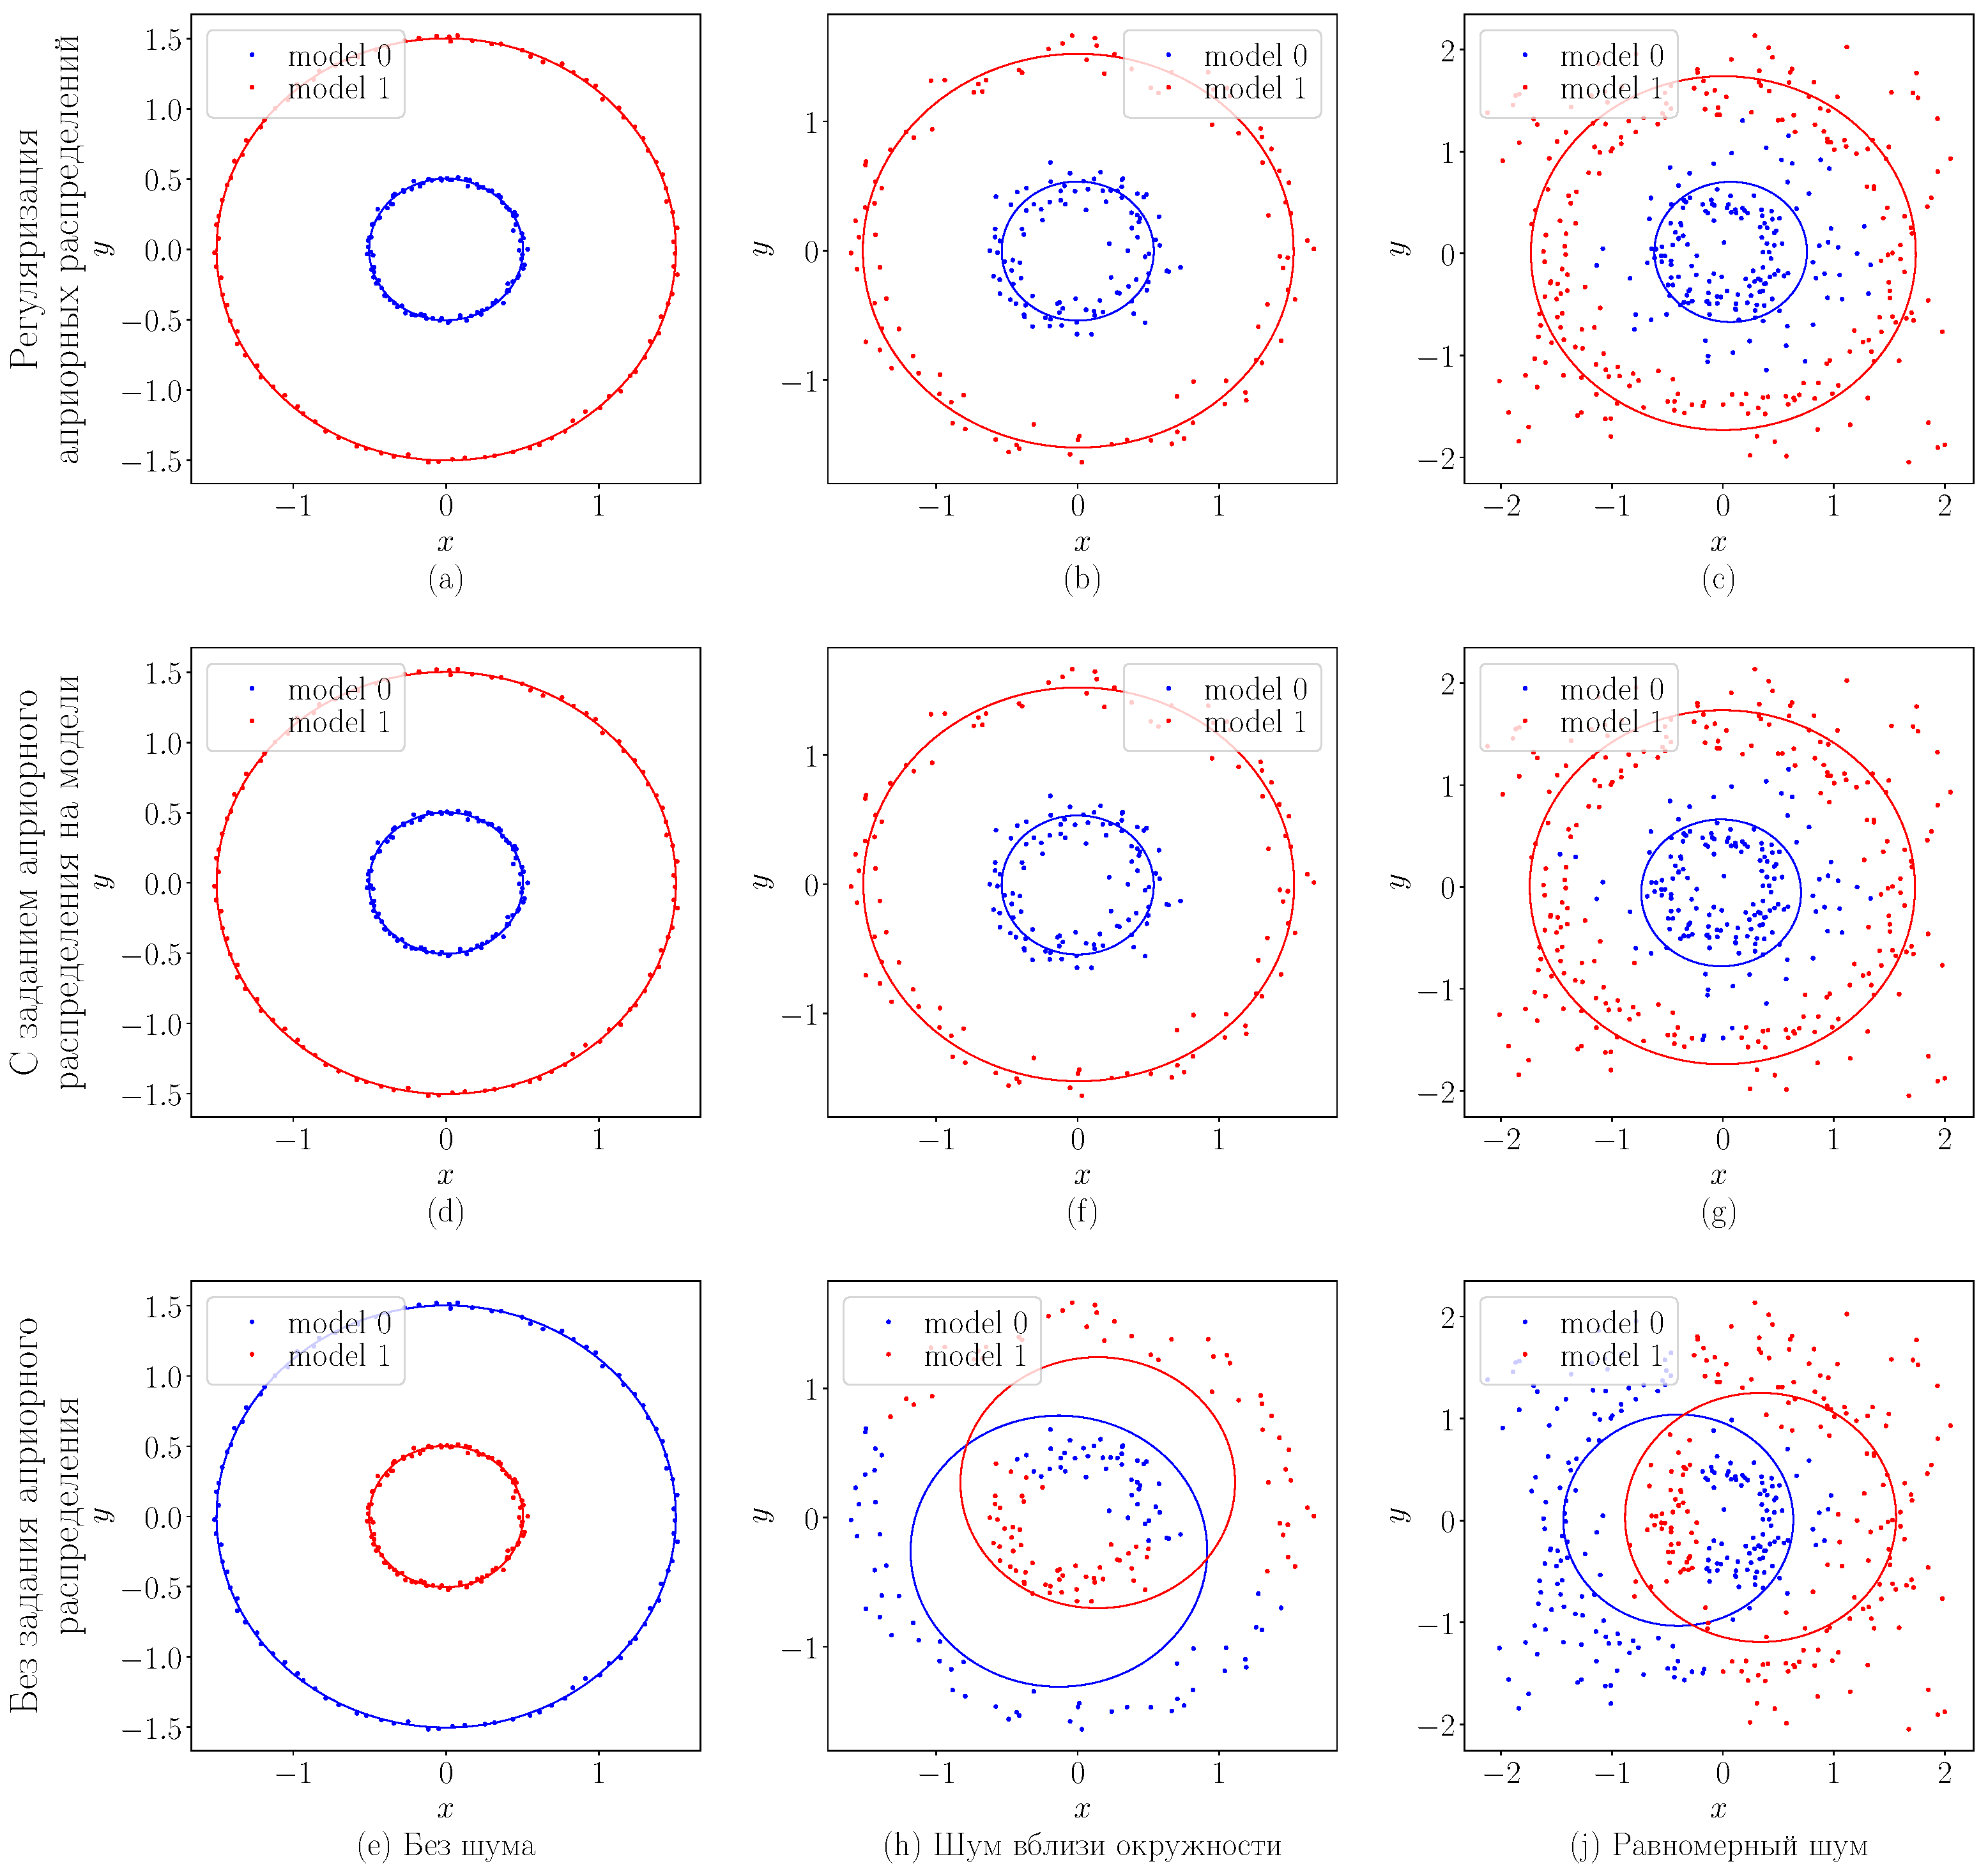
\includegraphics[height=0.9\textheight]{result/experiment_synthetic}
\end{center}

\end{frame}
%----------------------------------------------------------------------------------------------------------
\begin{frame}{Параметры локальных моделей в процессе обучения}
\justifying
\begin{center}
	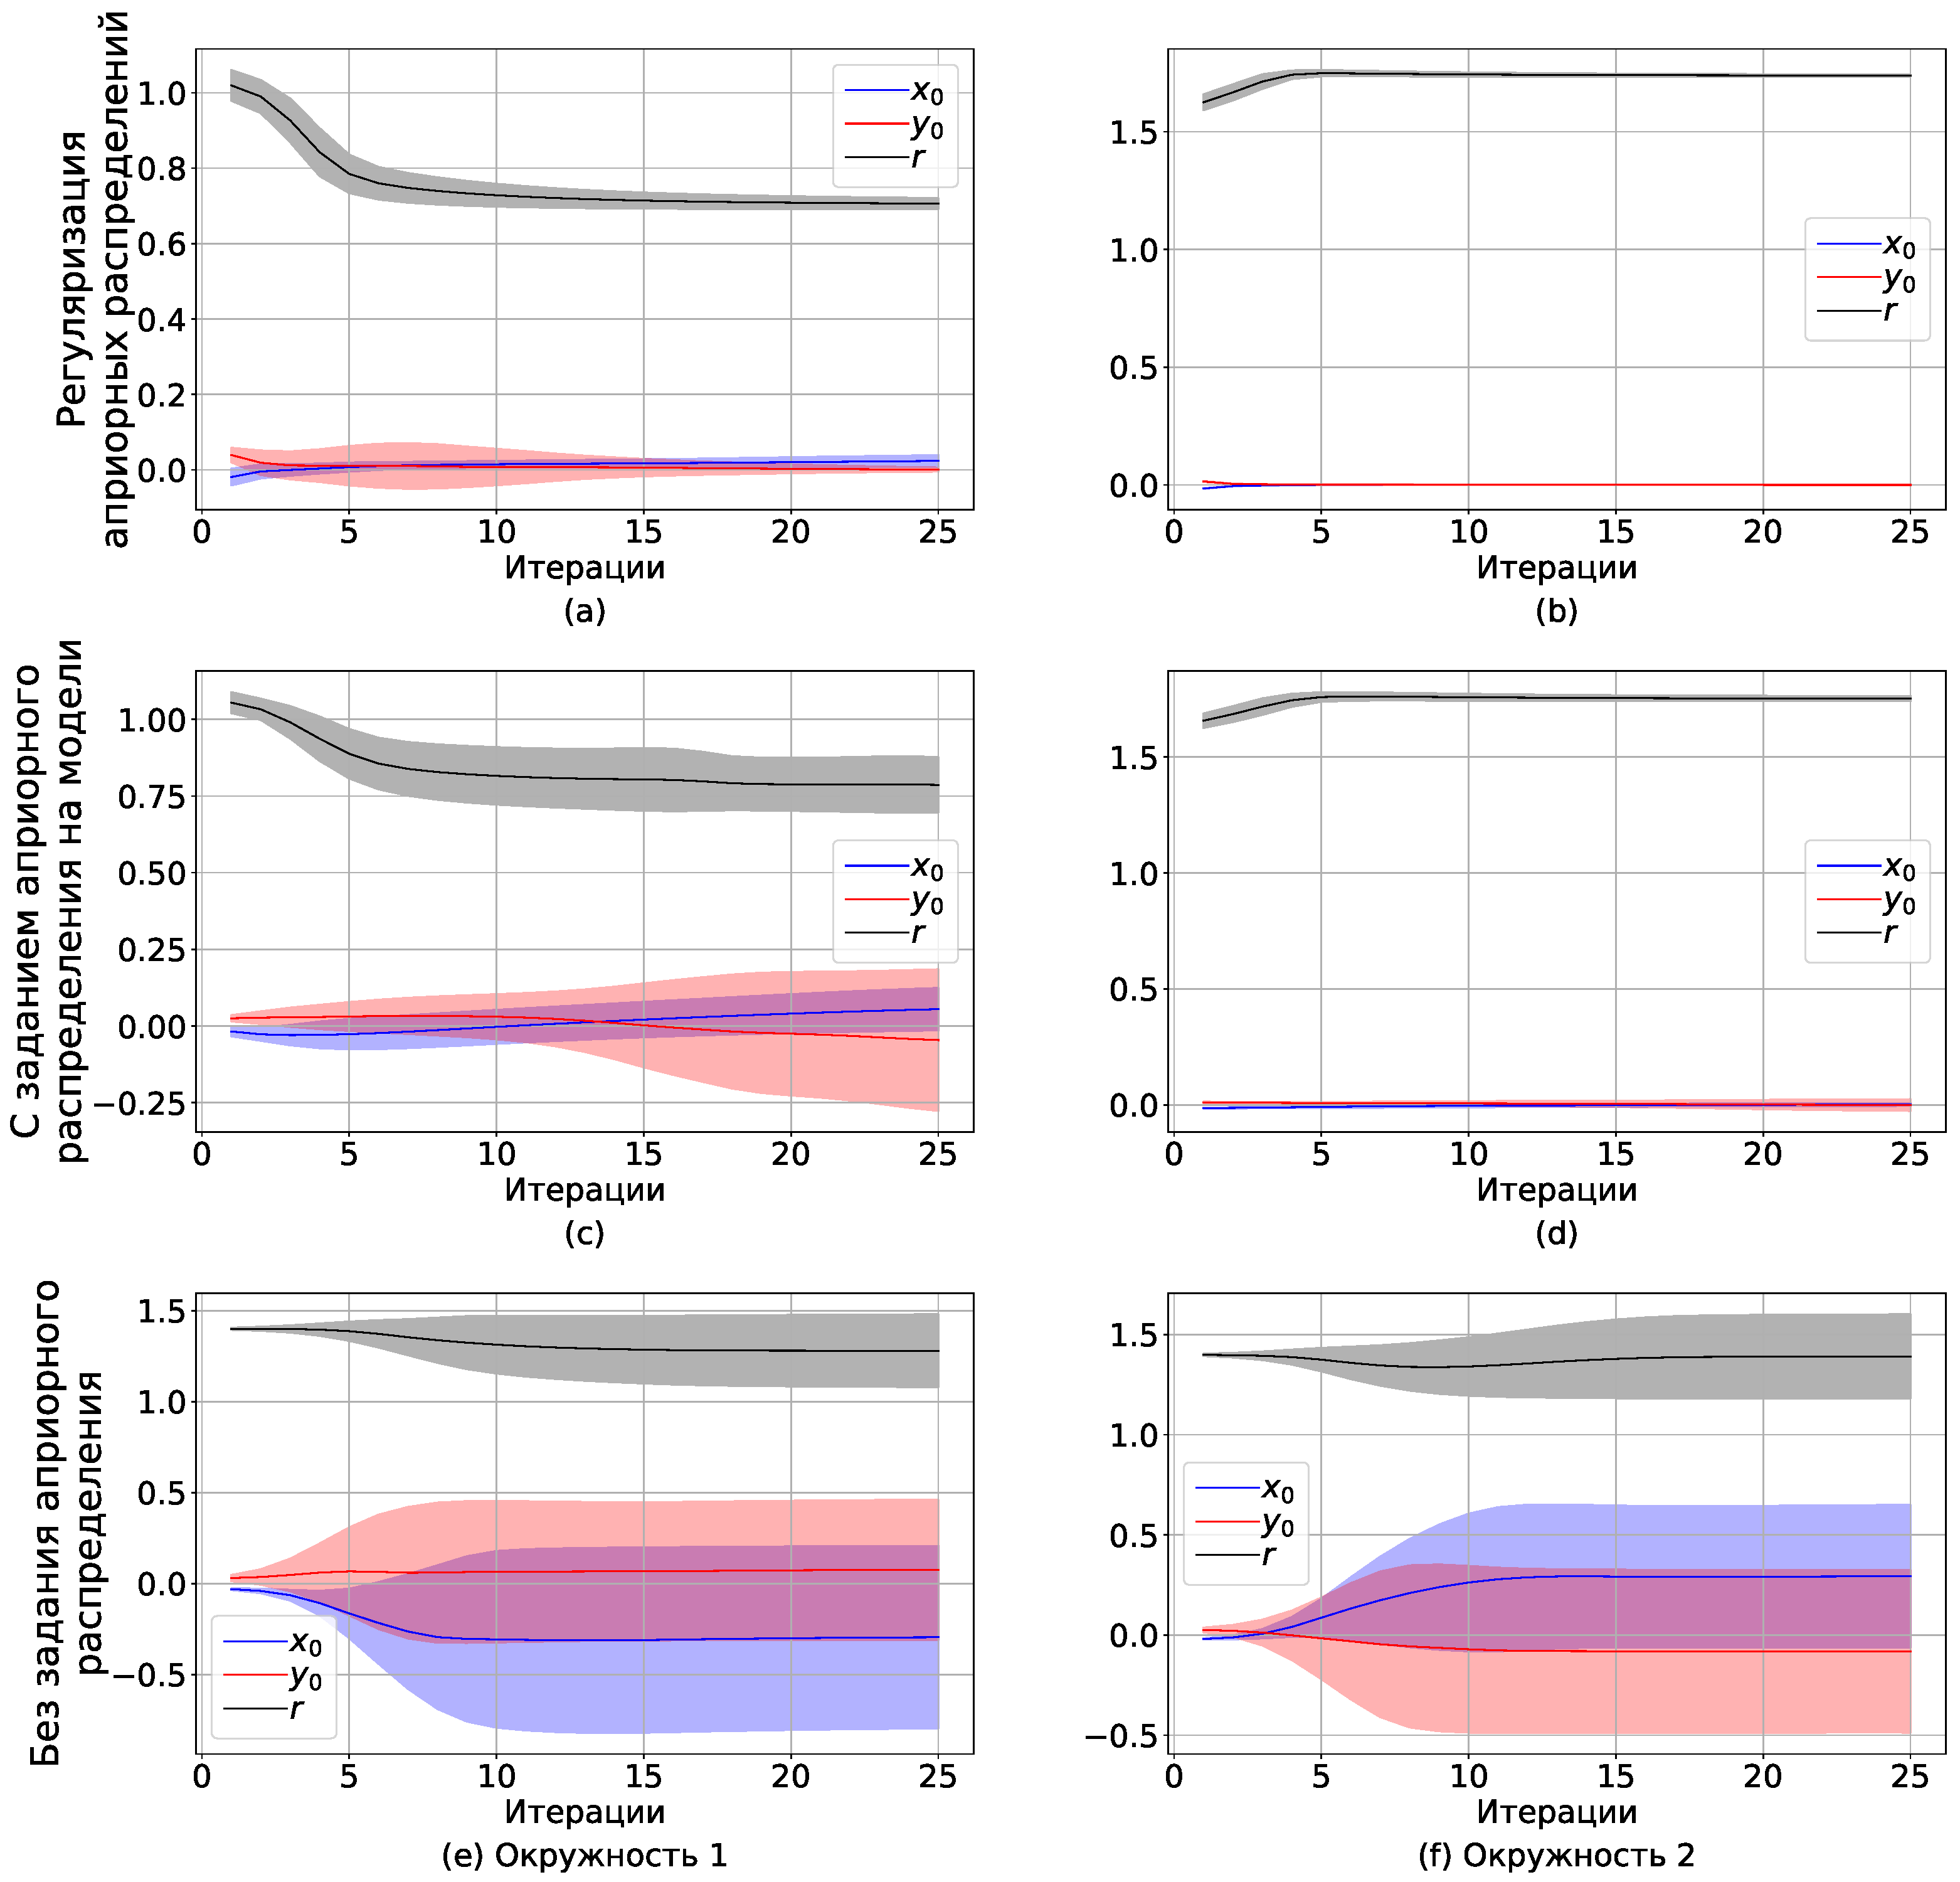
\includegraphics[height=0.9\textheight]{result/experiment_synthetic_param_progress}
\end{center}

\end{frame}
%----------------------------------------------------------------------------------------------------------
\begin{frame}{Обучения на синтетических данных}
\justifying
Регуляризация априорных распределений
\begin{center}
	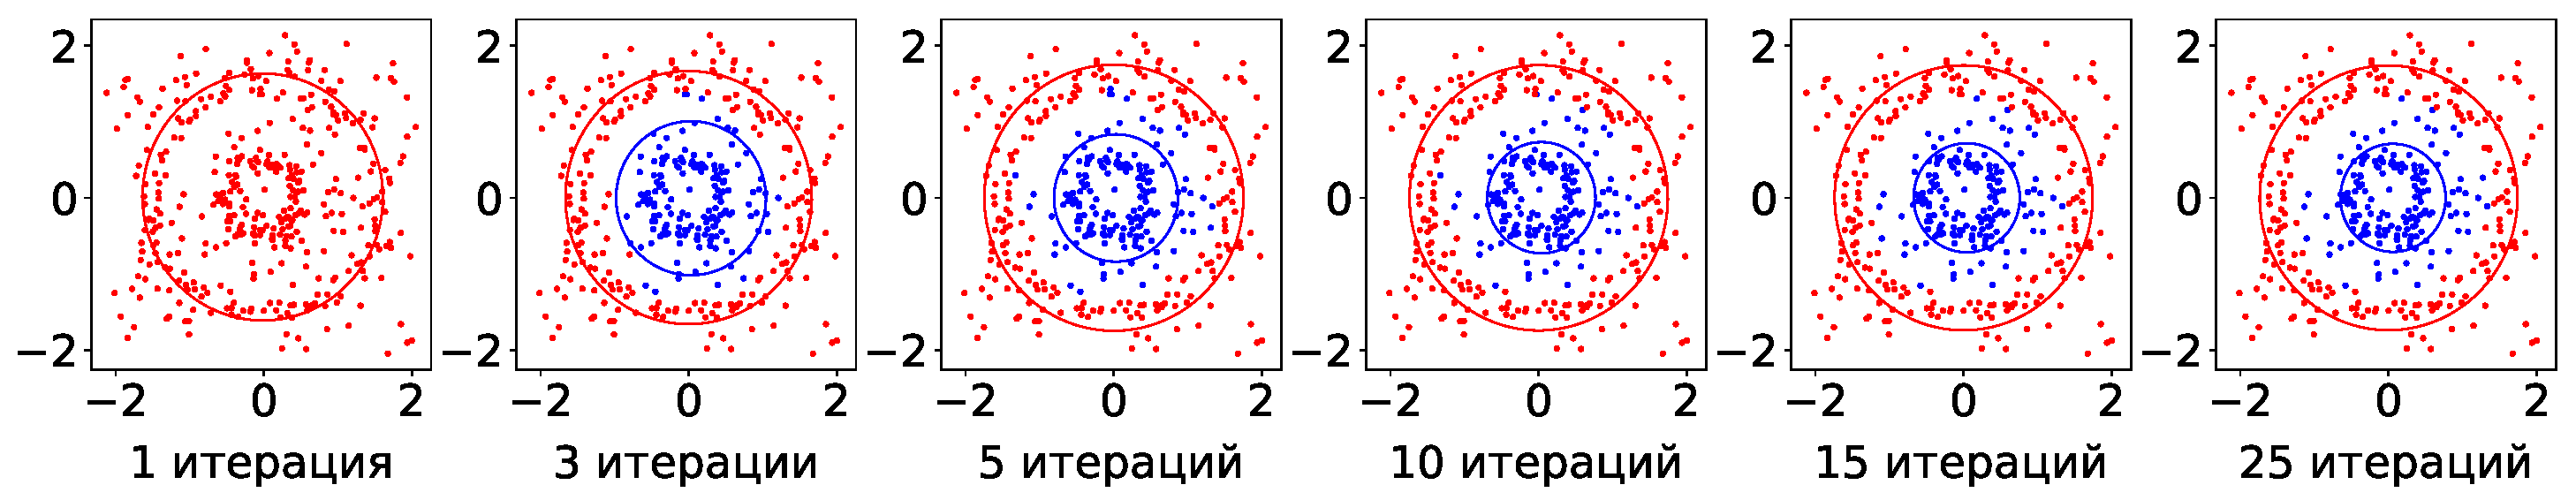
\includegraphics[width=0.95\textwidth]{result/experiment_synt_regular_progress}
\end{center}
С заданием априорного распределения на модели
\begin{center}
	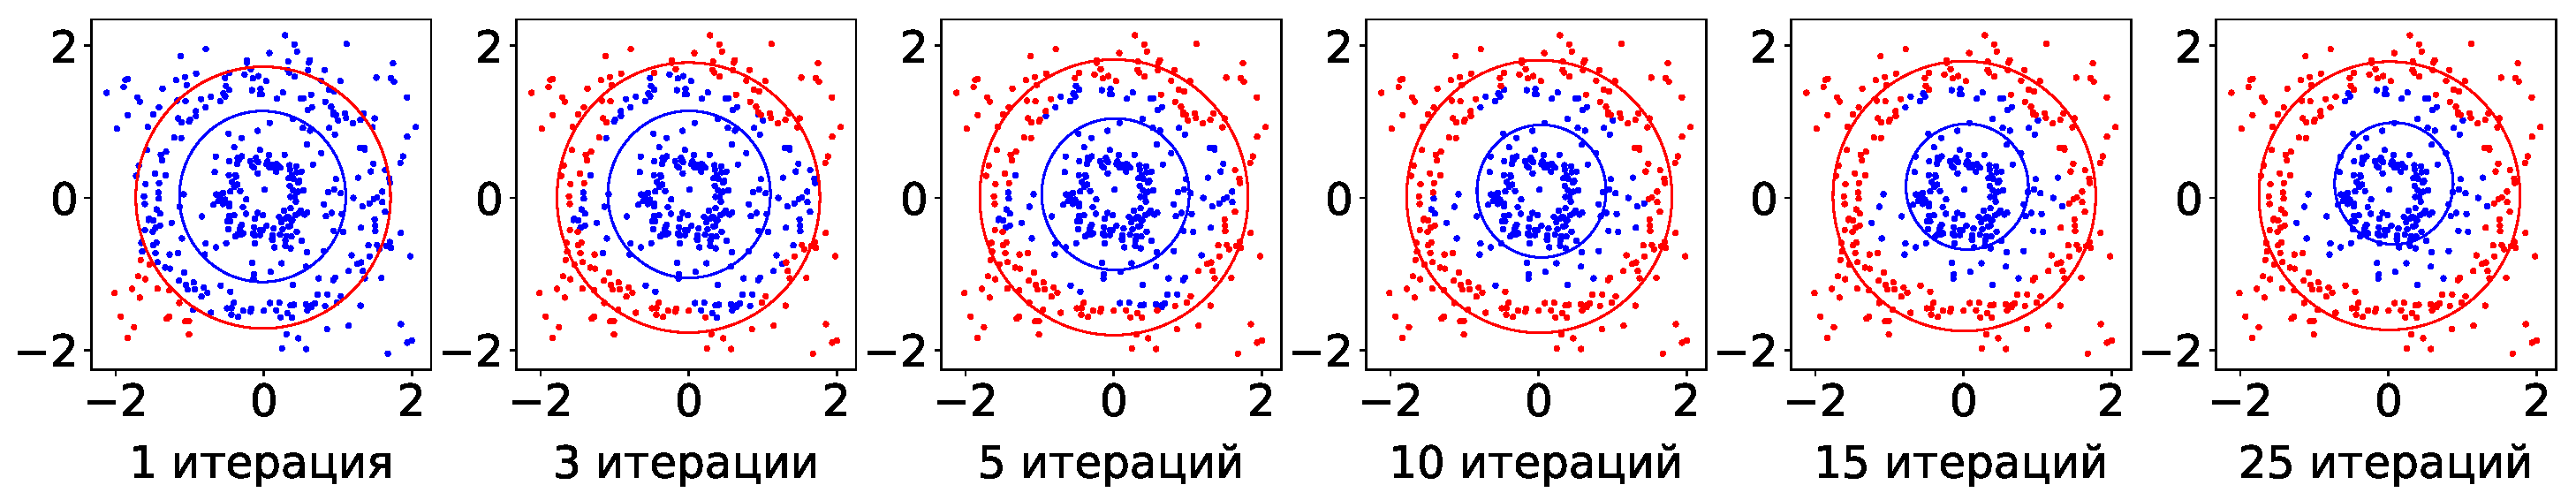
\includegraphics[width=0.95\textwidth]{result/experiment_synt_prior_progress}
\end{center}
Без задания априорного распределения
\begin{center}
	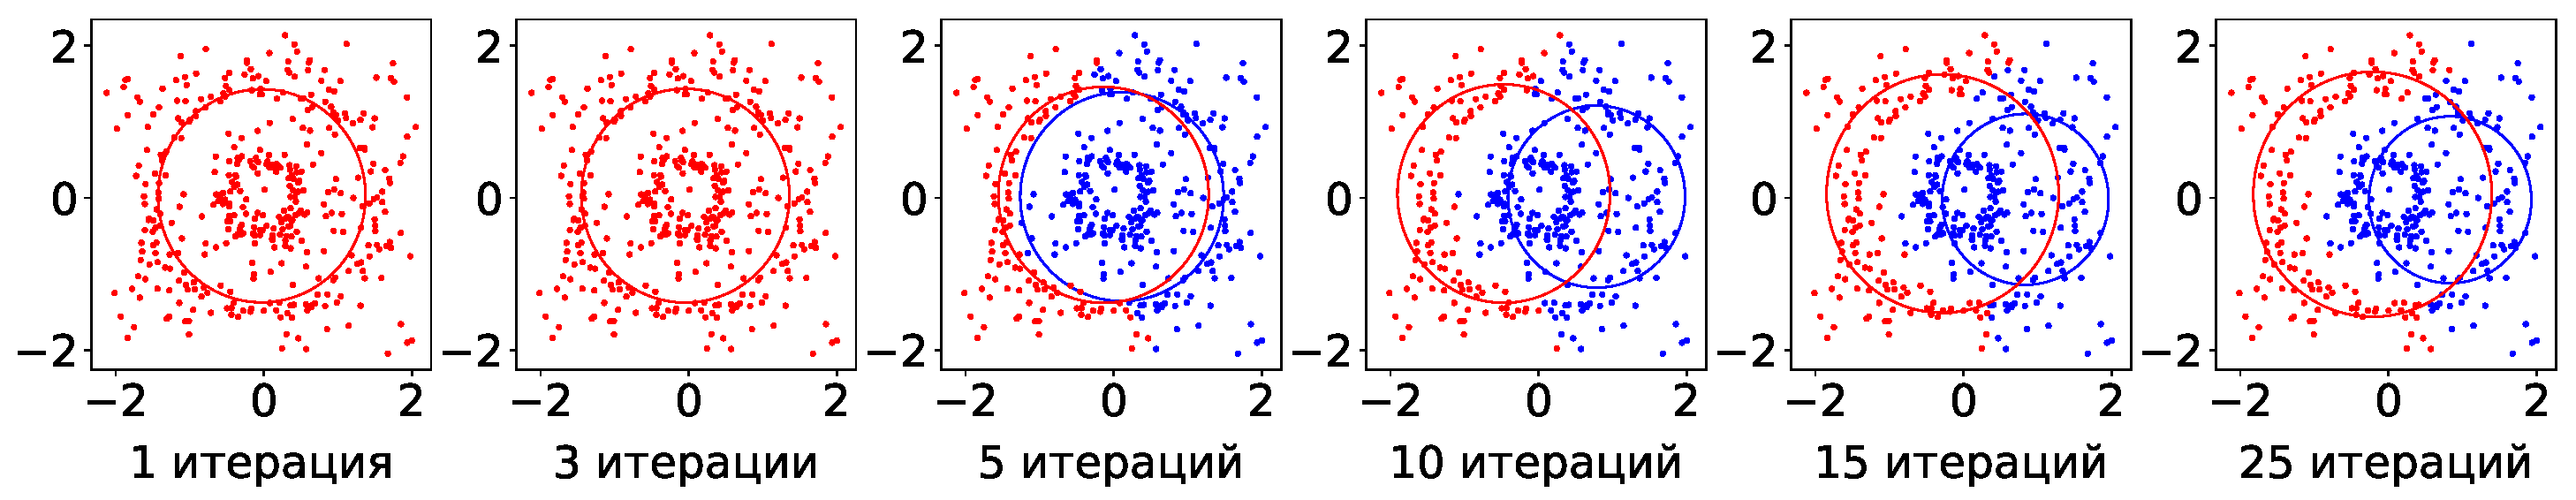
\includegraphics[width=0.95\textwidth]{result/experiment_synt_not_prior_progress}
\end{center}
\end{frame}
%----------------------------------------------------------------------------------------------------------
\begin{frame}{Анализ мультимоделей в зависимости от уровня шума}
\justifying
\begin{center}
	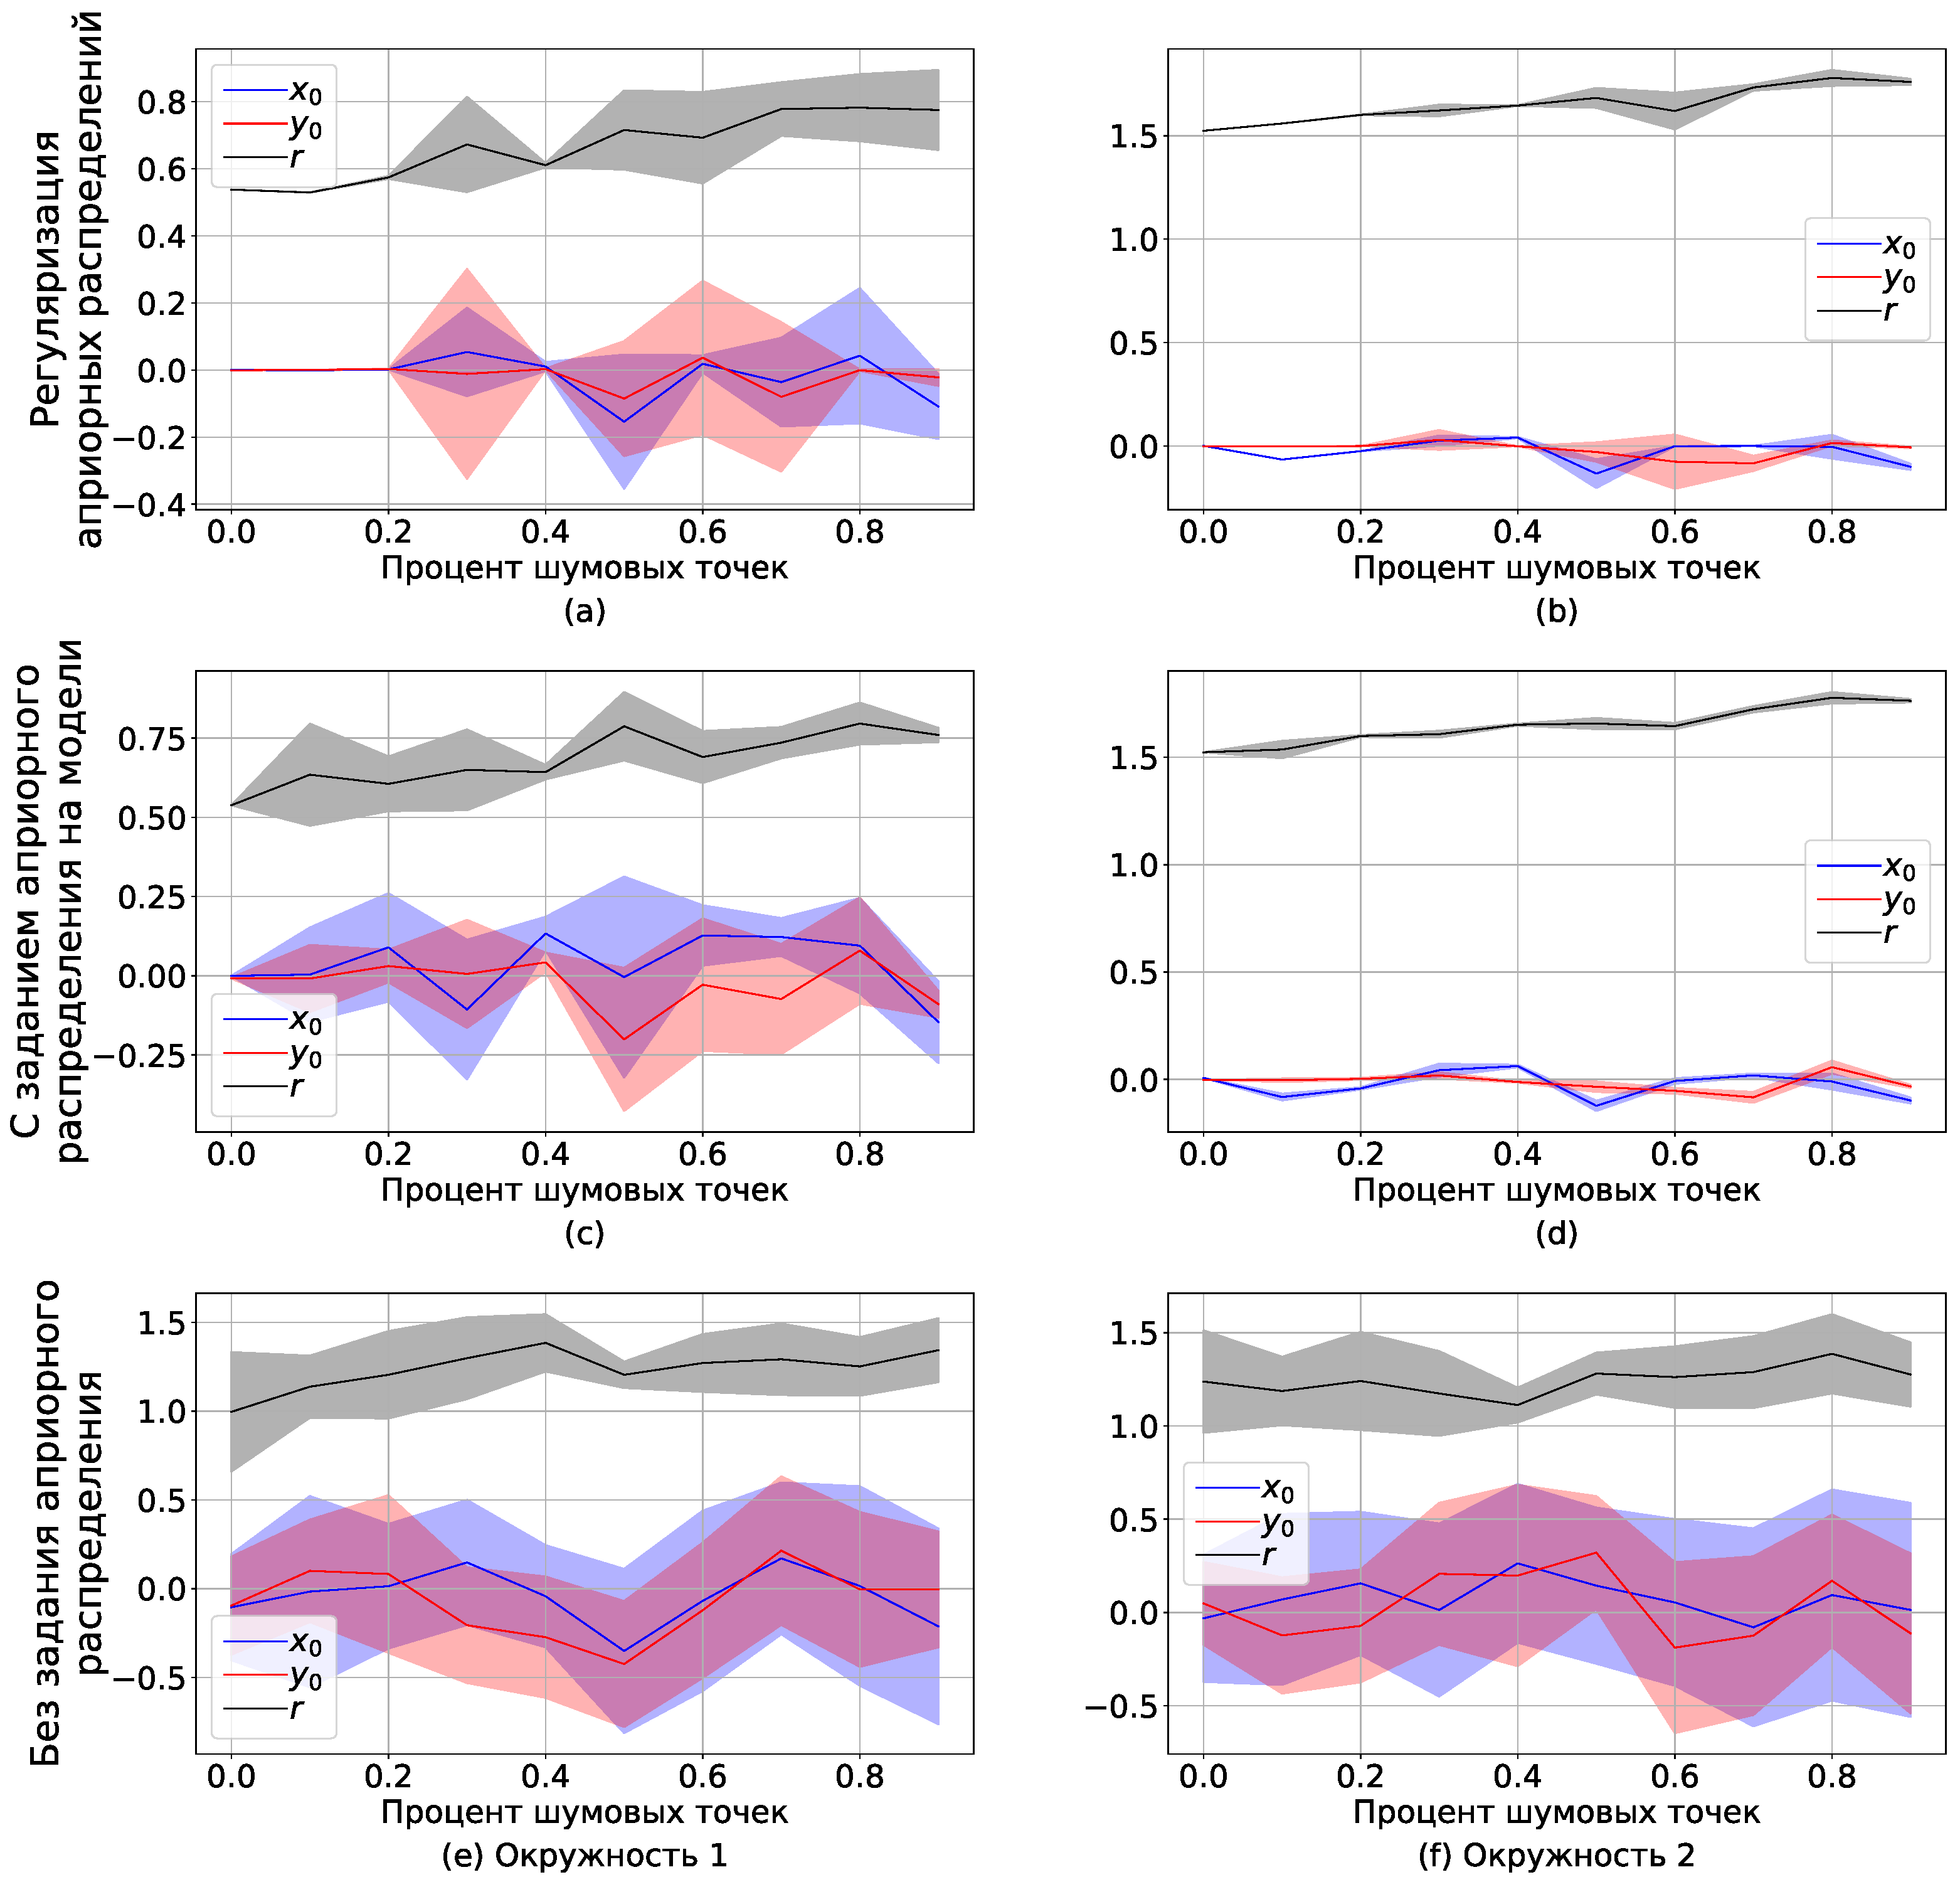
\includegraphics[height=0.9\textheight]{result/experiment_synthetic_param_progress_noise}
\end{center}

\end{frame}
%----------------------------------------------------------------------------------------------------------
\begin{frame}{Результаты на реальных данных}
\justifying
\begin{center}
	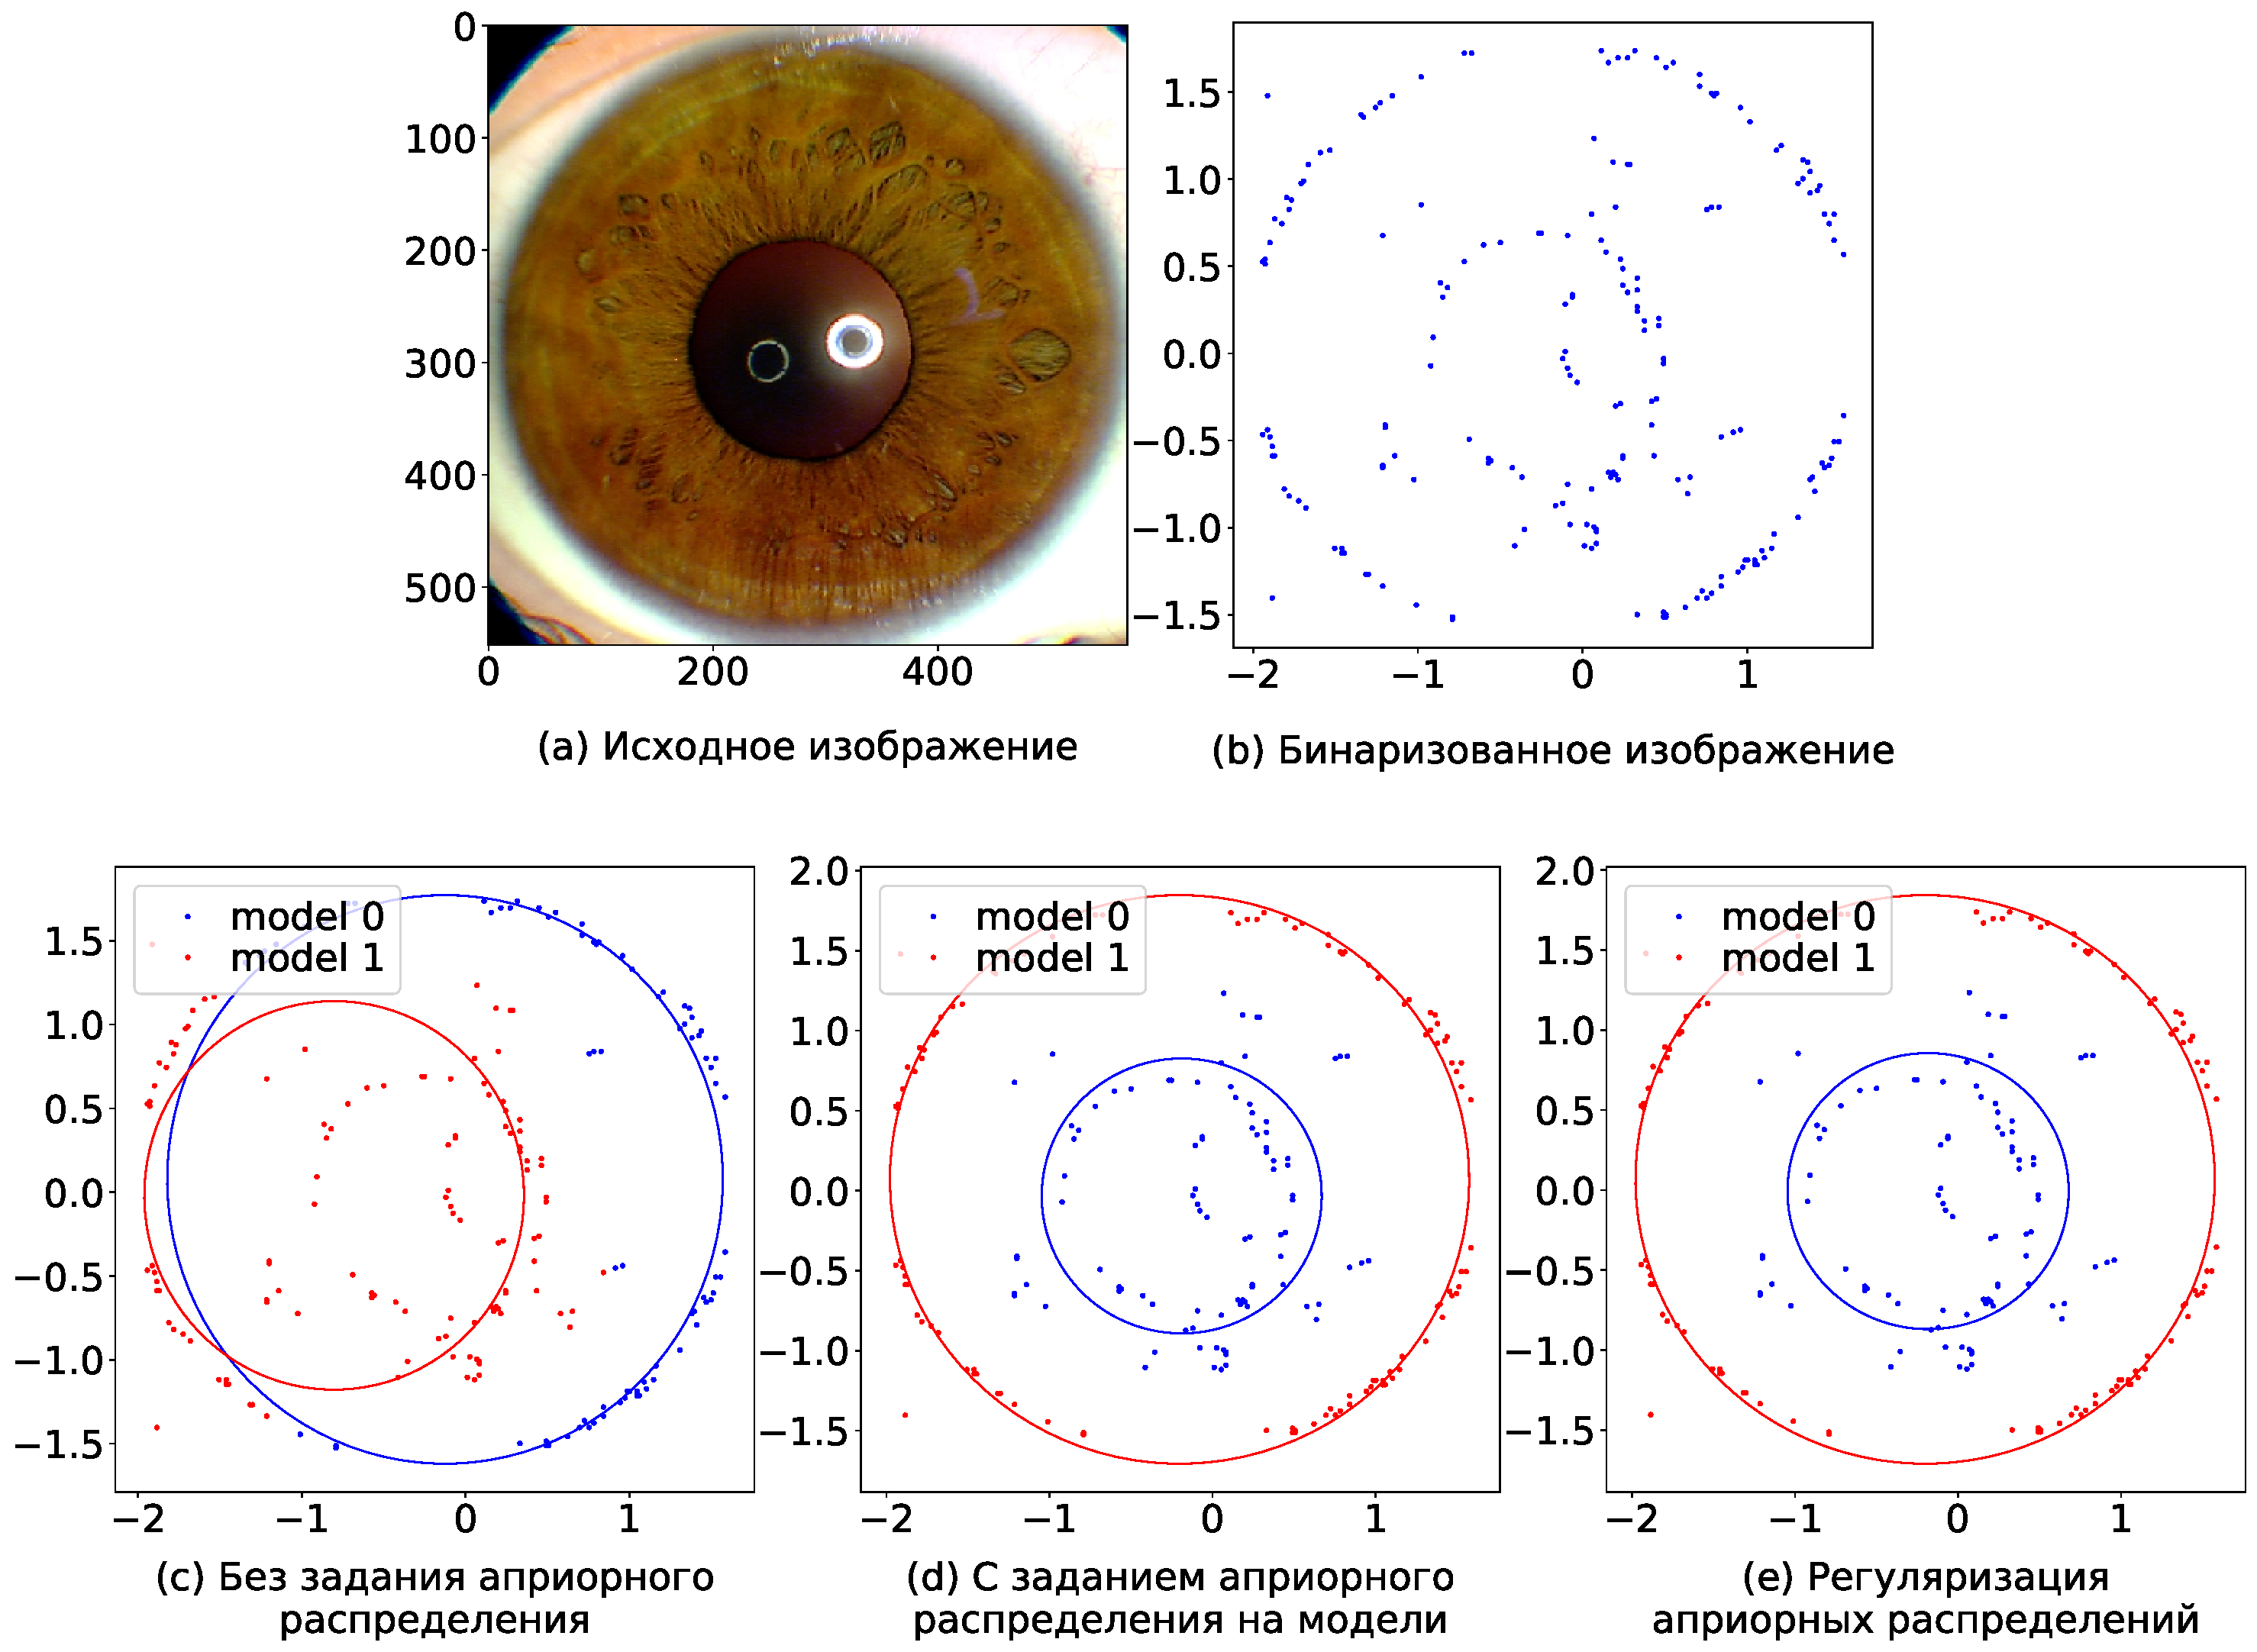
\includegraphics[height=0.9\textheight]{result/experiment_real_compare}
\end{center}

\end{frame}
%----------------------------------------------------------------------------------------------------------
\begin{frame}{Обучения на реальных данных}
\justifying
Регуляризация априорных распределений
\begin{center}
	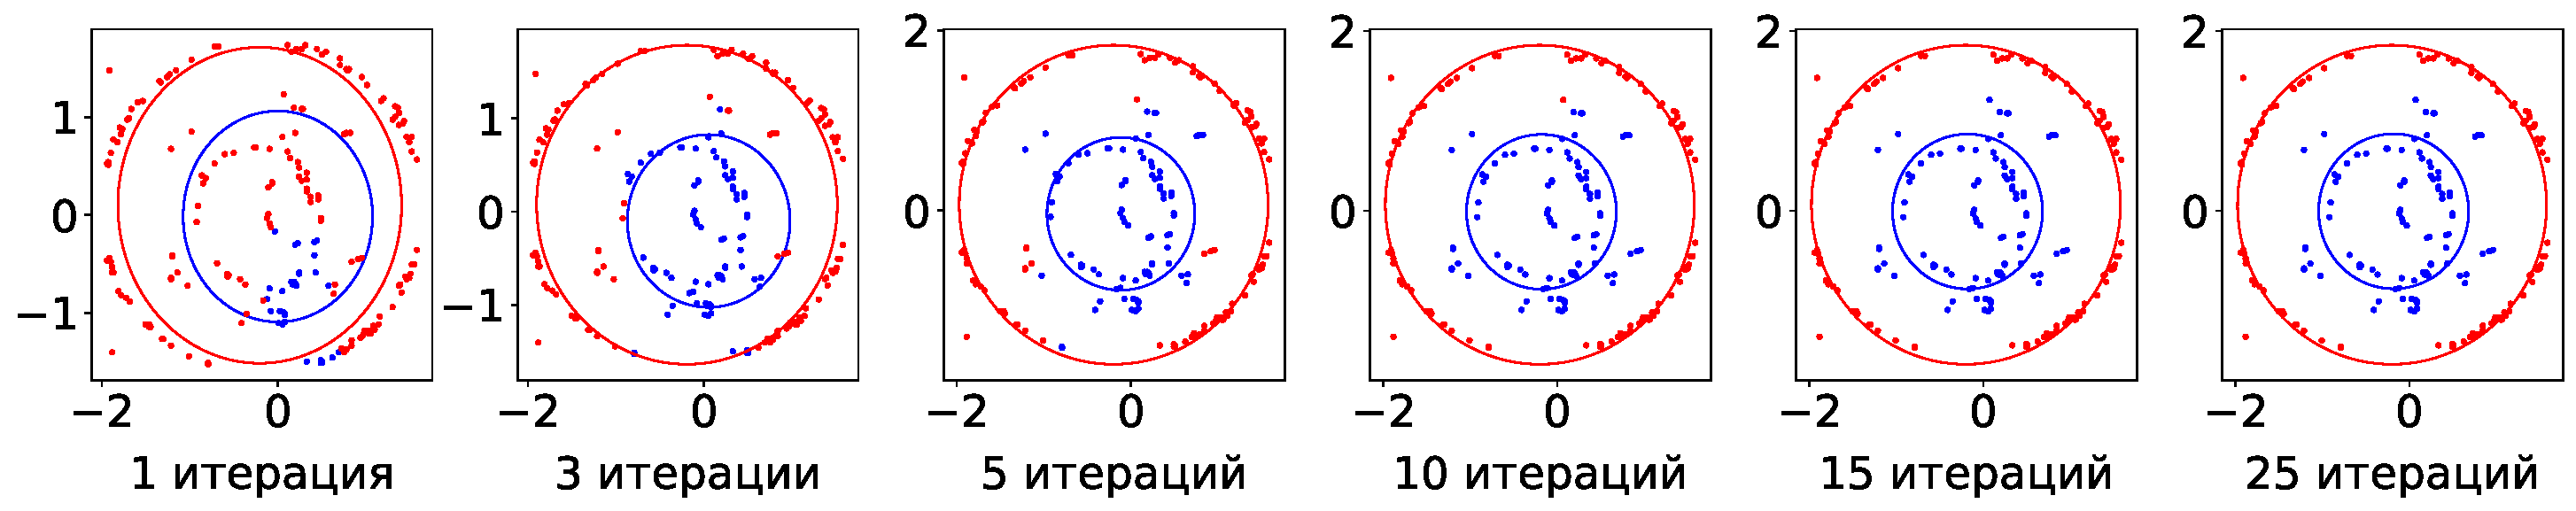
\includegraphics[width=0.95\textwidth]{result/experiment_real_regular}
\end{center}
С заданием априорного распределения на модели
\begin{center}
	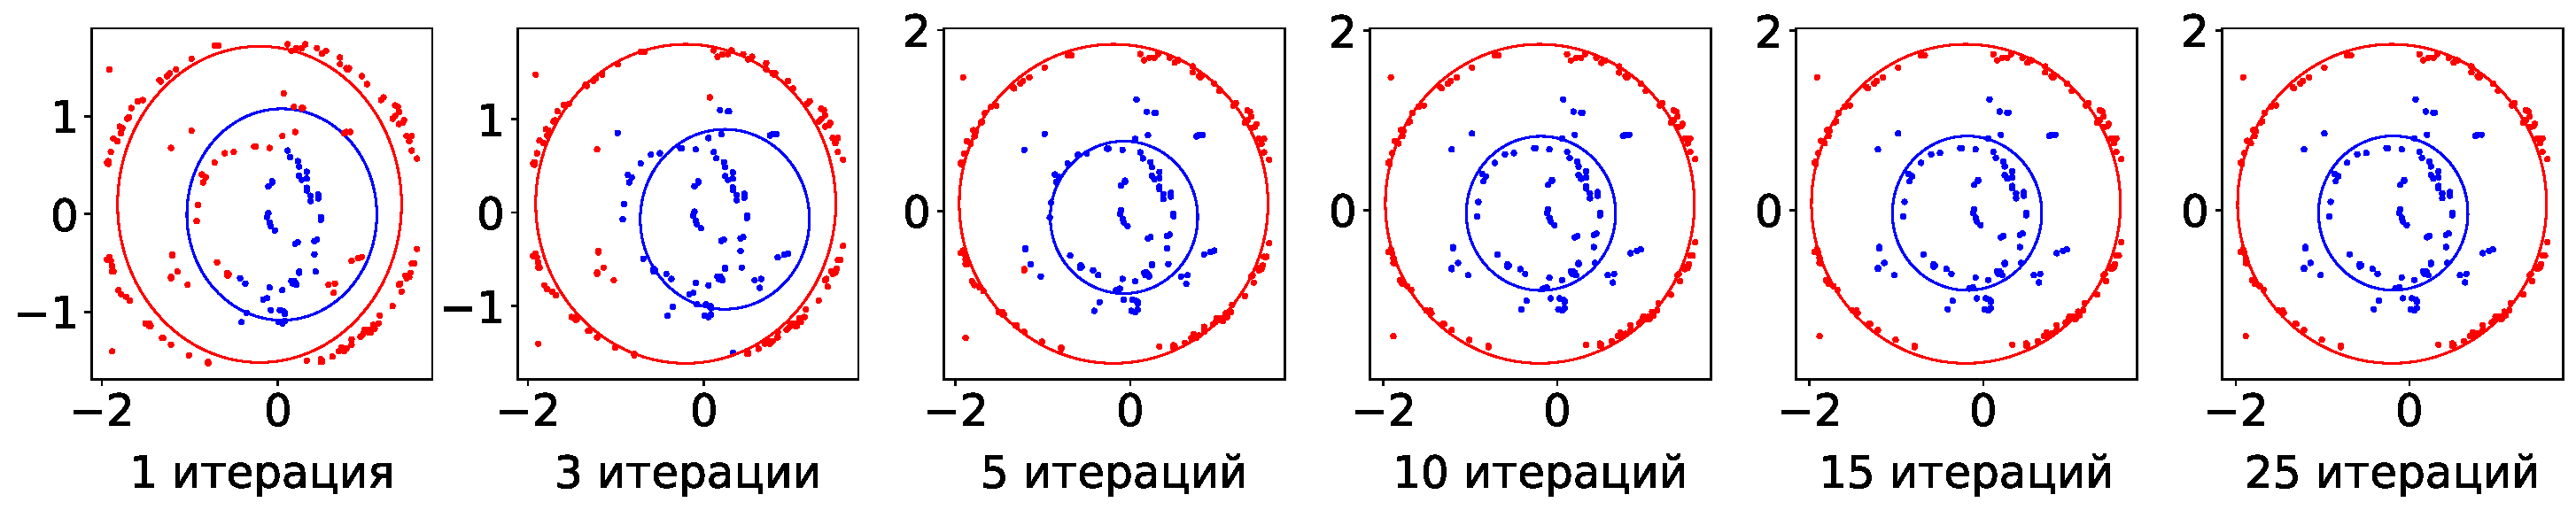
\includegraphics[width=0.95\textwidth]{result/experiment_real_prior}
\end{center}
Без задания априорного распределения
\begin{center}
	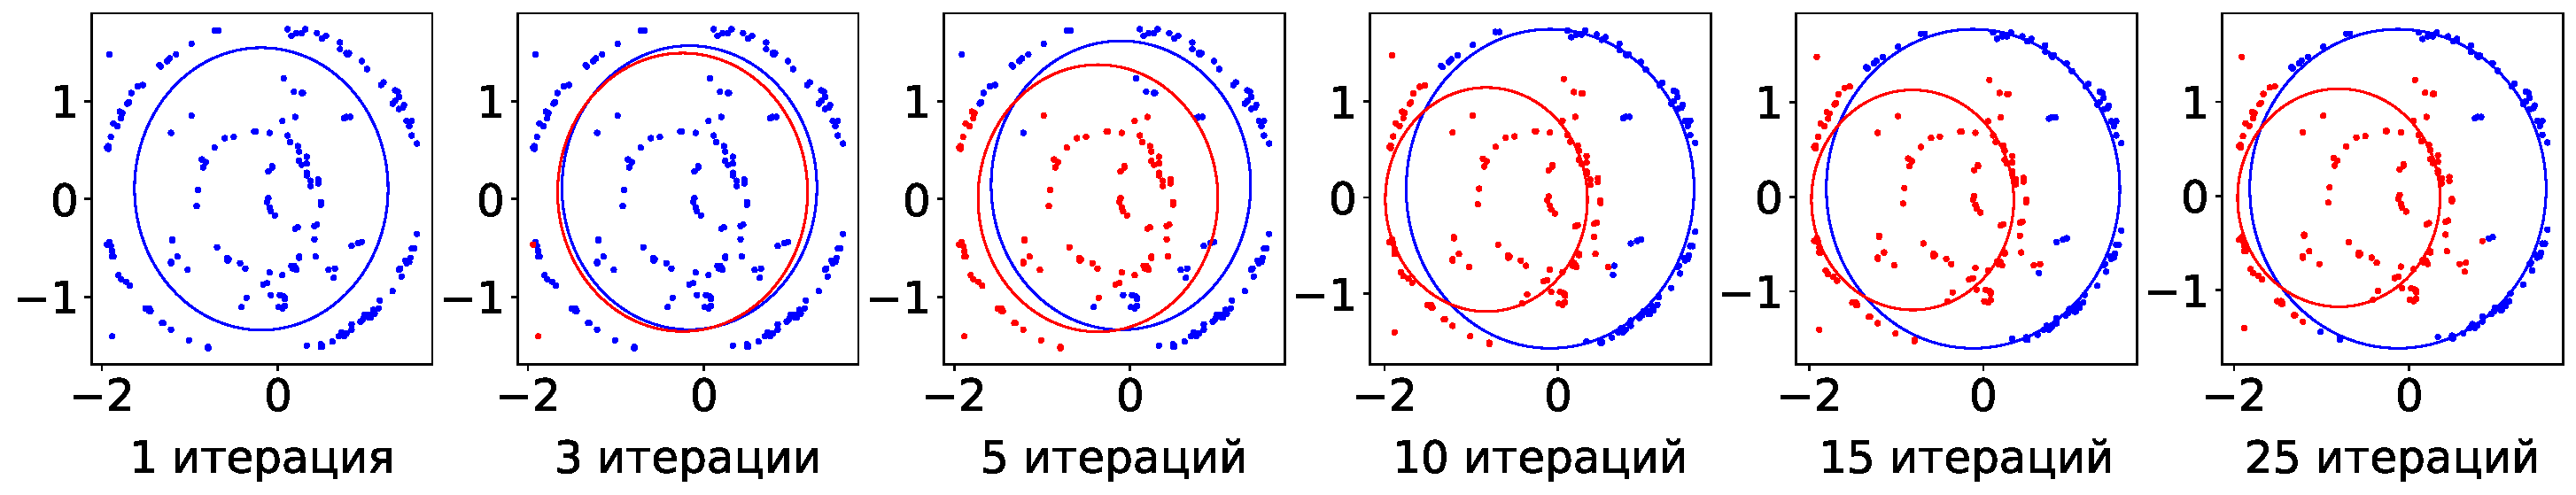
\includegraphics[width=0.95\textwidth]{result/experiment_real_not_prior}
\end{center}
\end{frame}
%----------------------------------------------------------------------------------------------------------
\begin{frame}{Вывод}
\justifying
Сделано:
	\begin{enumerate}
	\justifying
		\item Предложен метод поиска окружностей на бинарном изображении с различными априорными предположениями.
		\item Введено понятие регуляризации априорных распределений для улучшения качества мультимодели.
		\item В эксперименте показано, что задания регуляризации позволяет улучшить качество и устойчивость модели.
	\end{enumerate}

Планируется:
	\begin{enumerate}
	\justifying
		\item Улучшить мультимодель при помощи задания априорного распределения на шлюзовую функцию.
		\item Рассмотреть в качестве локальных моделей не только модели, которые описывают данные, а также модель, которая отвечает за шум в данных.
		\item Расширить класс локальных моделей с окружности до произвольной кривой второго порядка.
	\end{enumerate}	

\end{frame}
%----------------------------------------------------------------------------------------------------------

\begin{frame}{Постановка задачи обучения с экспертами}
\justifying
Пусть задано множество объектов~$\bm{\Omega}$, а также подмножество наблюдаемых объектов~$\bm{\Omega}'$
\begin{equation*}
\begin{aligned}
\bm{\Omega}'\subset\bm{\Omega},
\end{aligned}
\end{equation*}
где~$\left|\bm{\Omega}'\right|=N$.
Пусть для~$\bm{\Omega}$ задана некоторая экспертная информация~$\bm{E}\left(\bm{\Omega}\right)$.

На основе экспертной информации~$\bm{E}\left(\bm{\Omega}\right)$ введем отображения из множества объектов~$\bm{\Omega}$:
\begin{equation*}
\begin{aligned}
K_y^{\bm{E}\left(\bm{\Omega}\right)} :\bm{\Omega}\to \mathbb{R}, \quad K_x^{\bm{E}\left(\bm{\Omega}\right)} :\bm{\Omega}\to \mathbb{R}^{n},
\end{aligned}
\end{equation*}
где~$n$ количество признаков, причем предполагаем, что~$n\ll N$. Применив отображения~$K_x^{\bm{E}\left(\bm{\Omega}\right)}$ и~$K_y^{\bm{E}\left(\bm{\Omega}\right)}$ для множества наблюдаемых объектов~$\bm{\Omega}'$ получаем выборку:
\begin{equation*}
\begin{aligned}
\mathfrak{D}\left(\bm{\Omega}',\bm{E}\left(\bm{\Omega}\right)\right) = \{\left(\textbf{x}, y\right)|\textbf{x}=K_x^{\bm{E}\left(\bm{\Omega}\right)}\left(\omega\right),~y=K_y^{\bm{E}\left(\bm{\Omega}\right)}\left(\omega\right),~\forall \omega \in \bm{\Omega}'\}.
\end{aligned}
\end{equation*}

Предполагается, что существуют нетривиальные отображения~$K_y^{\bm{E}\left(\bm{\Omega}\right)}, K_x^{\bm{E}\left(\bm{\Omega}\right)}$, и~$\textbf{w}\in\mathbb{R}^{n}$, такие, что:
\begin{equation*}
\begin{aligned}
y \approx \textbf{x}^{\mathsf{T}}\textbf{w}, \quad \forall\left(\textbf{x}, y\right)\in\mathfrak{D}\left(\bm{\Omega}',\bm{E}\left(\bm{\Omega}\right)\right),
\end{aligned}
\end{equation*}
то есть получаем выборку, которая является задачей линейной регрессии по нахождению неизвестного вектора~$\textbf{w}$ (аналогично можно ввести задачу для логистической регрессии).

\end{frame}
%----------------------------------------------------------------------------------------------------------

\begin{frame}{Постановка задачи обучения с экспертами}
\justifying
В случае, когда экспертная информация представляется в виде объединения нескольких экспертов:
\begin{equation*}
\label{eq:st:5}
\begin{aligned}
\bm{E}\left(\bm{\Omega}\right) = \bm{E}_0\left(\bm{\Omega}\right)\cup\bm{E}_1\left(\bm{\Omega}_1\right)\cup\bm{E}_2\left(\bm{\Omega}_2\right)\cup\cdots\cup\bm{E}_K\left(\bm{\Omega}_K\right), \quad \cup_{i=k}^{K}\bm{\Omega}_k=\bm{\Omega}
\end{aligned}
\end{equation*}
в этом случае будем говорить о задаче смеси~$K$ экспертов. Каждая информация~$\bm{E}_k\left(\bm{\Omega}_k\right)$ описывает локальную информацию о каком-то подмножестве объектов~$\bm{\Omega}_k$ для всех~$k=\overline{1...K}$. Информация эксперта~$\bm{E}_0\left(\bm{\Omega}\right)$ описывает глобальную информацию о всем множестве объектов~$\bm{\Omega}$.

В случае задачи смеси~$K$ экспертов вводятся отображения:
\begin{equation*}
\label{eq:st:6}
\begin{aligned}
K_y^{\bm{E}_1\left(\bm{\Omega}_1\right)} :\bm{\Omega}\to \mathbb{R}, \quad K_x^{\bm{E}_1\left(\bm{\Omega}_1\right)} :\bm{\Omega}\to \mathbb{R}^{n_1},\\
\cdots\\
K_y^{\bm{E}_K\left(\bm{\Omega}_K\right)} :\bm{\Omega}\to \mathbb{R}, \quad K_x^{\bm{E}_K\left(\bm{\Omega}_K\right)} :\bm{\Omega}\to \mathbb{R}^{n_K},\\
\end{aligned}
\end{equation*}
где получаем множество отображений во множество локальных моделей, в которых учтены информации от каждого эксперта.

Также, как в и задаче одного эксперта вводится предположения, что каждая локальная модель является линейной:
\begin{equation*}
\label{eq:st:7}
\begin{aligned}
\forall k\in\{1,\cdots K\}, \quad y \approx \textbf{x}^{\mathsf{T}}\textbf{w}_k, \quad \forall\left(\textbf{x}, y\right)\in\mathfrak{D}\left(\bm{\Omega}'_{k},\bm{E}\left(\bm{\Omega}_k\right)\right).
\end{aligned}
\end{equation*}

\end{frame}
%----------------------------------------------------------------------------------------------------------

\begin{frame}{Постановка задачи обучения с экспертами}
\justifying
Заметим, что истинного разбиения~$\bm{\Omega}$ на множества~$\{\bm{\Omega}_k\}_{k=1}^{K}$ нету. Рассмотрим вектор функцию~$\bm{\pi}$:
\begin{equation*}
\label{eq:st:8}
\begin{aligned}
\bm{\pi}:\bm{\Omega}\to \mathbb{R}^{K}, \quad \sum_{k=1}^{K}\pi_{k}\left(\omega\right)=1,~\forall\omega\in\bm{\Omega},
\end{aligned}
\end{equation*}
где~$\bm{\pi}$ назовем шлюзовой функцией.

Предположим, что все~$\left\{\left(K_x^{\bm{E}_k\left(\bm{\Omega}_k\right)}, K_y^{\bm{E}_k\left(\bm{\Omega}_k\right)}\right)\right\}_{k=1}^{K}$ являются заданными отображениями. Используя локальные модели, построим глобальную мультимодель, которая описывает все множество объектов~$\bm{\Omega}$:
\begin{equation*}
\label{eq:st:9}
\begin{aligned}
\sum_{\omega \in \bm{\Omega}'}\sum_{k=1}^{K}\pi_{k}\left(\omega, \textbf{V}\right)\left(K_y^{\bm{E}_k\left(\bm{\Omega}_k\right)}\left(\omega\right) - \textbf{w}_{k}^{\mathsf{T}}K_x^{\bm{E}_k\left(\bm{\Omega}_k\right)}\left(\omega\right) \right)^2 + R\left(\textbf{V}, \textbf{W}, \bm{E}\left(\bm{\Omega}\right)\right) \to \min_{\textbf{V}, \textbf{W}}
\end{aligned}
\end{equation*}
где~$\textbf{W}=[\textbf{w}_1^\mathsf{T}, \cdots, \textbf{w}_K^{\mathsf{T}}]$, а~$R\left(\textbf{V}, \textbf{W}, \bm{E}\left(\bm{\Omega}\right)\right)$ является некоторой регуляризацией параметров, которая также основывается на экспертной информации, $\textbf{V}$~--- параметры шлюзовой функции.
\end{frame}
%----------------------------------------------------------------------------------------------------------

\begin{frame}{Пример}
\justifying

\begin{figure}[h!t]\center
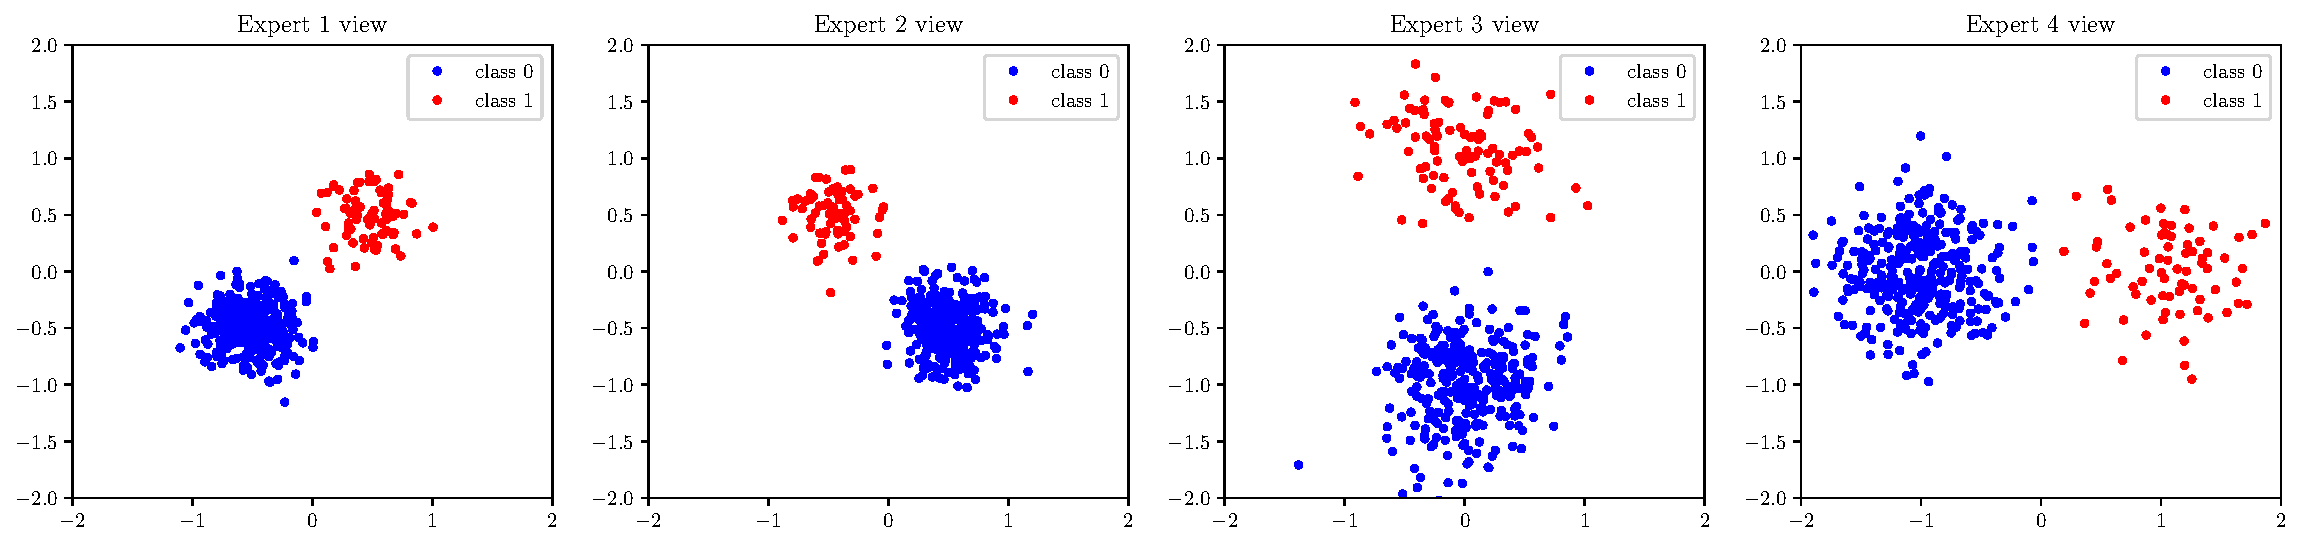
\includegraphics[width=1.0\textwidth]{figures/expert_example}
\label{intro:fig1}
\end{figure}

\end{frame}
%----------------------------------------------------------------------------------------------------------

\begin{frame}{Задача поиска кривых второго порядка: результат аппроксимации}
\justifying

\begin{figure}[h!t]\center
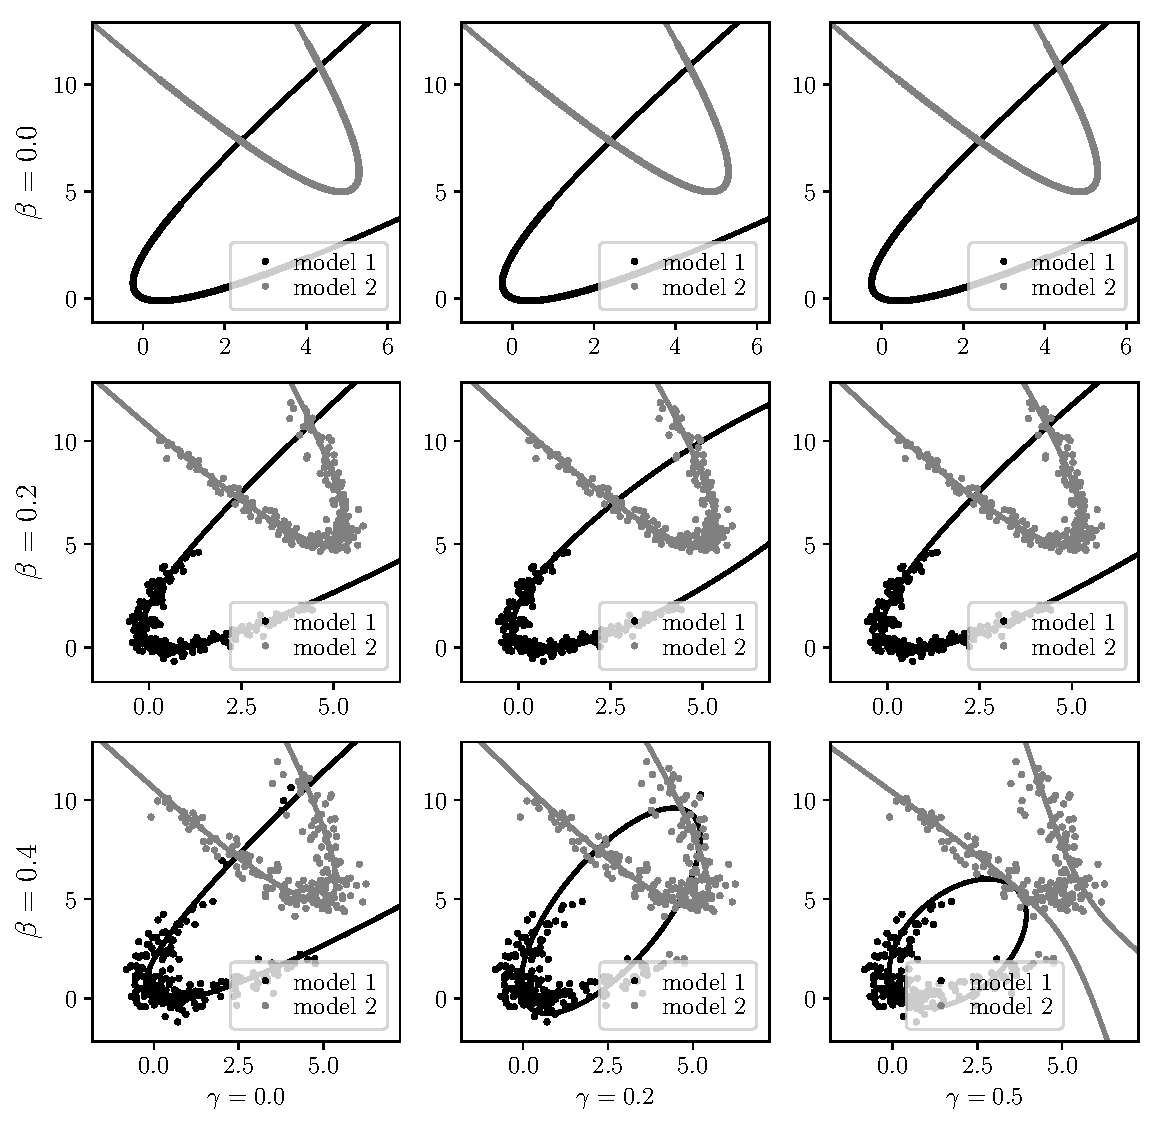
\includegraphics[width=0.75\textwidth]{figures/beta_gamma}
\caption{Результат аппроксимации для данных с разным уровнем шума~$\beta$ и от дисперсии априорного распределения~$\gamma$}
\end{figure}

\end{frame}
%----------------------------------------------------------------------------------------------------------

\begin{frame}{Задача поиска кривых второго порядка: от уровня шума}
\justifying

\begin{figure}[h!t]\center
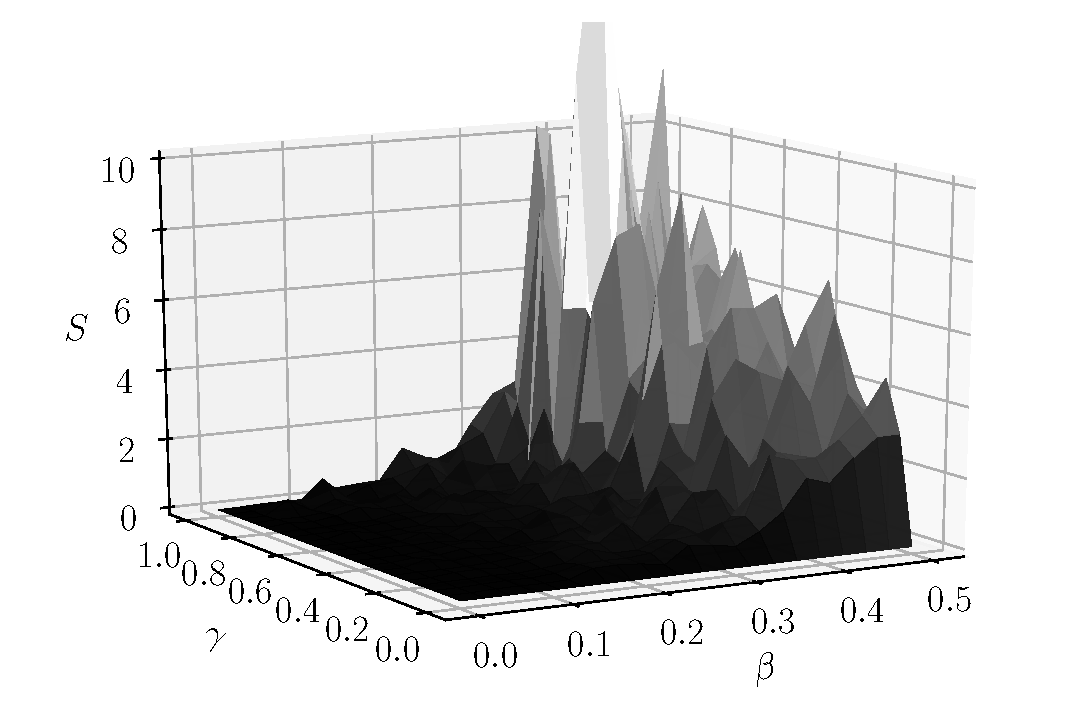
\includegraphics[width=0.75\textwidth]{figures/3dplot}
\end{figure}

\end{frame}

\end{document} 